% Options for packages loaded elsewhere
\PassOptionsToPackage{unicode}{hyperref}
\PassOptionsToPackage{hyphens}{url}
\PassOptionsToPackage{dvipsnames,svgnames,x11names}{xcolor}
%
\documentclass[
  letterpaper,
  DIV=11,
  numbers=noendperiod]{scrartcl}

\usepackage{amsmath,amssymb}
\usepackage{iftex}
\ifPDFTeX
  \usepackage[T1]{fontenc}
  \usepackage[utf8]{inputenc}
  \usepackage{textcomp} % provide euro and other symbols
\else % if luatex or xetex
  \usepackage{unicode-math}
  \defaultfontfeatures{Scale=MatchLowercase}
  \defaultfontfeatures[\rmfamily]{Ligatures=TeX,Scale=1}
\fi
\usepackage{lmodern}
\ifPDFTeX\else  
    % xetex/luatex font selection
\fi
% Use upquote if available, for straight quotes in VerbatimWithBreaks environments
\IfFileExists{upquote.sty}{\usepackage{upquote}}{}
\IfFileExists{microtype.sty}{% use microtype if available
  \usepackage[]{microtype}
  \UseMicrotypeSet[protrusion]{basicmath} % disable protrusion for tt fonts
}{}
\makeatletter
\@ifundefined{KOMAClassName}{% if non-KOMA class
  \IfFileExists{parskip.sty}{%
    \usepackage{parskip}
  }{% else
    \setlength{\parindent}{0pt}
    \setlength{\parskip}{6pt plus 2pt minus 1pt}}
}{% if KOMA class
  \KOMAoptions{parskip=half}}
\makeatother
\usepackage{xcolor}
\setlength{\emergencystretch}{3em} % prevent overfull lines
\setcounter{secnumdepth}{-\maxdimen} % remove section numbering
% Make \paragraph and \subparagraph free-standing
\makeatletter
\ifx\paragraph\undefined\else
  \let\oldparagraph\paragraph
  \renewcommand{\paragraph}{
    \@ifstar
      \xxxParagraphStar
      \xxxParagraphNoStar
  }
  \newcommand{\xxxParagraphStar}[1]{\oldparagraph*{#1}\mbox{}}
  \newcommand{\xxxParagraphNoStar}[1]{\oldparagraph{#1}\mbox{}}
\fi
\ifx\subparagraph\undefined\else
  \let\oldsubparagraph\subparagraph
  \renewcommand{\subparagraph}{
    \@ifstar
      \xxxSubParagraphStar
      \xxxSubParagraphNoStar
  }
  \newcommand{\xxxSubParagraphStar}[1]{\oldsubparagraph*{#1}\mbox{}}
  \newcommand{\xxxSubParagraphNoStar}[1]{\oldsubparagraph{#1}\mbox{}}
\fi
\makeatother

\usepackage{color}
\usepackage{fancyvrb}
\newcommand{\VerbBar}{|}
\newcommand{\VERB}{\Verb[commandchars=\\\{\}]}
\DefineVerbatimEnvironment{Highlighting}{Verbatim}{commandchars=\\\{\}}
% Add ',fontsize=\small' for more characters per line
\usepackage{framed} % Para o ambiente Shaded
\usepackage{seqsplit} % Para quebrar texto longo
\usepackage{minted} % Para destaque de sintaxe
\usepackage{fvextra} % Para quebra de linha
\usepackage{xcolor} % Para cores
\definecolor{shadecolor}{RGB}{241,243,245}
\newenvironment{Shaded}{\begin{snugshade}}{\end{snugshade}}
% Redefinição do VerbatimWithBreaks para incluir quebra de linha
\newenvironment{VerbatimWithBreaksWithBreaks}{
    \begin{snugshade} % Início do sombreamento
    \begingroup
    \let\oldtext\text
    \renewcommand{\text}[1]{\seqsplit{##1}}
}{
    \endgroup
    \end{snugshade} % Fim do sombreamento
}
% Definir o ambiente Highlighting com fvextra
\DefineVerbatimEnvironment{Highlighting}{Verbatim}{%
    breaklines=true,       % Habilita quebra de linha
    commandchars=\\\{\}   % Mantém a interpretação de caracteres especiais
}
\usepackage{makeidx}
\newcommand{\AlertTok}[1]{\textcolor[rgb]{0.68,0.00,0.00}{#1}}
\newcommand{\AnnotationTok}[1]{\textcolor[rgb]{0.37,0.37,0.37}{#1}}
\newcommand{\AttributeTok}[1]{\textcolor[rgb]{0.40,0.45,0.13}{#1}}
\newcommand{\BaseNTok}[1]{\textcolor[rgb]{0.68,0.00,0.00}{#1}}
\newcommand{\BuiltInTok}[1]{\textcolor[rgb]{0.00,0.23,0.31}{#1}}
\newcommand{\CharTok}[1]{\textcolor[rgb]{0.13,0.47,0.30}{#1}}
\newcommand{\CommentTok}[1]{\textcolor[rgb]{0.37,0.37,0.37}{#1}}
\newcommand{\CommentVarTok}[1]{\textcolor[rgb]{0.37,0.37,0.37}{\textit{#1}}}
\newcommand{\ConstantTok}[1]{\textcolor[rgb]{0.56,0.35,0.01}{#1}}
\newcommand{\ControlFlowTok}[1]{\textcolor[rgb]{0.00,0.23,0.31}{\textbf{#1}}}
\newcommand{\DataTypeTok}[1]{\textcolor[rgb]{0.68,0.00,0.00}{#1}}
\newcommand{\DecValTok}[1]{\textcolor[rgb]{0.68,0.00,0.00}{#1}}
\newcommand{\DocumentationTok}[1]{\textcolor[rgb]{0.37,0.37,0.37}{\textit{#1}}}
\newcommand{\ErrorTok}[1]{\textcolor[rgb]{0.68,0.00,0.00}{#1}}
\newcommand{\ExtensionTok}[1]{\textcolor[rgb]{0.00,0.23,0.31}{#1}}
\newcommand{\FloatTok}[1]{\textcolor[rgb]{0.68,0.00,0.00}{#1}}
\newcommand{\FunctionTok}[1]{\textcolor[rgb]{0.28,0.35,0.67}{#1}}
\newcommand{\ImportTok}[1]{\textcolor[rgb]{0.00,0.46,0.62}{#1}}
\newcommand{\InformationTok}[1]{\textcolor[rgb]{0.37,0.37,0.37}{#1}}
\newcommand{\KeywordTok}[1]{\textcolor[rgb]{0.00,0.23,0.31}{\textbf{#1}}}
\newcommand{\NormalTok}[1]{\textcolor[rgb]{0.00,0.23,0.31}{#1}}
\newcommand{\OperatorTok}[1]{\textcolor[rgb]{0.37,0.37,0.37}{#1}}
\newcommand{\OtherTok}[1]{\textcolor[rgb]{0.00,0.23,0.31}{#1}}
\newcommand{\PreprocessorTok}[1]{\textcolor[rgb]{0.68,0.00,0.00}{#1}}
\newcommand{\RegionMarkerTok}[1]{\textcolor[rgb]{0.00,0.23,0.31}{#1}}
\newcommand{\SpecialCharTok}[1]{\textcolor[rgb]{0.37,0.37,0.37}{#1}}
\newcommand{\SpecialStringTok}[1]{\textcolor[rgb]{0.13,0.47,0.30}{#1}}
\newcommand{\StringTok}[1]{\textcolor[rgb]{0.13,0.47,0.30}{#1}}
\newcommand{\VariableTok}[1]{\textcolor[rgb]{0.07,0.07,0.07}{#1}}
\newcommand{\VerbatimStringTok}[1]{\textcolor[rgb]{0.13,0.47,0.30}{#1}}
\newcommand{\WarningTok}[1]{\textcolor[rgb]{0.37,0.37,0.37}{\textit{#1}}}

\providecommand{\tightlist}{%
  \setlength{\itemsep}{0pt}\setlength{\parskip}{0pt}}\usepackage{longtable,booktabs,array}
\usepackage{calc} % for calculating minipage widths
% Correct order of tables after \paragraph or \subparagraph
\usepackage{etoolbox}
\makeatletter
\patchcmd\longtable{\par}{\if@noskipsec\mbox{}\fi\par}{}{}
\makeatother
% Allow footnotes in longtable head/foot
\IfFileExists{footnotehyper.sty}{\usepackage{footnotehyper}}{\usepackage{footnote}}
\makesavenoteenv{longtable}
\usepackage{graphicx}
\makeatletter
\newsavebox\pandoc@box
\newcommand*\pandocbounded[1]{% scales image to fit in text height/width
  \sbox\pandoc@box{#1}%
  \Gscale@div\@tempa{\textheight}{\dimexpr\ht\pandoc@box+\dp\pandoc@box\relax}%
  \Gscale@div\@tempb{\linewidth}{\wd\pandoc@box}%
  \ifdim\@tempb\p@<\@tempa\p@\let\@tempa\@tempb\fi% select the smaller of both
  \ifdim\@tempa\p@<\p@\scalebox{\@tempa}{\usebox\pandoc@box}%
  \else\usebox{\pandoc@box}%
  \fi%
}
% Set default figure placement to htbp
\def\fps@figure{htbp}
\makeatother

\KOMAoption{captions}{tableheading}
\makeatletter
\@ifpackageloaded{caption}{}{\usepackage{caption}}
\AtBeginDocument{%
\ifdefined\contentsname
  \renewcommand*\contentsname{Table of contents}
\else
  \newcommand\contentsname{Table of contents}
\fi
\ifdefined\listfigurename
  \renewcommand*\listfigurename{List of Figures}
\else
  \newcommand\listfigurename{List of Figures}
\fi
\ifdefined\listtablename
  \renewcommand*\listtablename{List of Tables}
\else
  \newcommand\listtablename{List of Tables}
\fi
\ifdefined\figurename
  \renewcommand*\figurename{Figure}
\else
  \newcommand\figurename{Figure}
\fi
\ifdefined\tablename
  \renewcommand*\tablename{Table}
\else
  \newcommand\tablename{Table}
\fi
}
\@ifpackageloaded{float}{}{\usepackage{float}}
\floatstyle{ruled}
\@ifundefined{c@chapter}{\newfloat{codelisting}{h}{lop}}{\newfloat{codelisting}{h}{lop}[chapter]}
\floatname{codelisting}{Listing}
\newcommand*\listoflistings{\listof{codelisting}{List of Listings}}
\makeatother
\makeatletter
\makeatother
\makeatletter
\@ifpackageloaded{caption}{}{\usepackage{caption}}
\@ifpackageloaded{subcaption}{}{\usepackage{subcaption}}
\makeatother

\usepackage{bookmark}

\IfFileExists{xurl.sty}{\usepackage{xurl}}{} % add URL line breaks if available
\urlstyle{same} % disable monospaced font for URLs
\hypersetup{
  colorlinks=true,
  linkcolor={blue},
  filecolor={Maroon},
  citecolor={Blue},
  urlcolor={Blue},
  pdfcreator={LaTeX via pandoc}}


\author{Mateus Sales Bentes}
\date{31-03-1997}

\makeindex

\begin{document}

Instalando as bibbliotecas necessárias.

\begin{Shaded}
\begin{Highlighting}[]
\OperatorTok{\%}\NormalTok{pip install datasets fasttext nltk pyspark}
\end{Highlighting}
\end{Shaded}

\begin{enumerate}
\def\labelenumi{\arabic{enumi}.}
\tightlist
\item
  Objetivo \index{Objetivo}
\end{enumerate}

O projeto atendeu ao objetivo principal de identificar e classificar
postagens do Bluesky em diferentes categorias temáticas. Essa análise é
relevante porque permite compreender os principais temas discutidos na
plataforma, suas características textuais e sua distribuição temporal.
As perguntas de pesquisa foram abordadas de forma sistemática:

Perguntas da Pesquisa

\begin{VerbatimWithBreaks}
1. Quais são os principais temas discutidos no Bluesky?
    Através da análise exploratória e da criação de categorias utilizando palavras-chave, foi possível identificar temas como Política, Esportes, Videogames e Guerra.

2. Quais características textuais diferenciam cada categoria?
     O pré-processamento de texto revelou diferenças significativas entre as categorias, como o uso de hashtags específicas e menções.

3. Quais temas são mais recorrentes e qual sua distribuição temporal?
    A dimensão Tempo permitiu análises sazonais e identificação de horários de pico para determinados tópicos.

4. É possível prever com boa precisão o tema de uma postagem usando aprendizado de máquina?
    Embora ainda não tenha sido implementado um modelo de aprendizado de máquina, o pipeline de limpeza e organização dos dados já está preparado para treinar modelos como Naive Bayes, SVM ou redes neurais.
\end{VerbatimWithBreaks}

\begin{enumerate}
\def\labelenumi{\arabic{enumi}.}
\setcounter{enumi}{1}
\tightlist
\item
  Coleta de Dados \index{Coleta de Dados}
\end{enumerate}

Os dados utilizados neste estudo foram obtidos a partir do dataset ``Two
Million Bluesky Posts'', disponível na plataforma Hugging Face. Esse
dataset contém um grande volume de postagens extraídas da rede social
Bluesky, incluindo os seguintes atributos:

\begin{VerbatimWithBreaks}
Texto da postagem
Data de criação
Identificador do autor
Presença de imagens
Respostas a outras postagens
\end{VerbatimWithBreaks}

A coleta foi realizada utilizando a biblioteca datasets da Hugging Face,
garantindo um acesso rápido e eficiente aos dados. O código para
importação foi:

\begin{Shaded}
\begin{Highlighting}[]
\ImportTok{import}\NormalTok{ datasets}
\ImportTok{from}\NormalTok{ datasets }\ImportTok{import}\NormalTok{ load\_dataset}

\NormalTok{ds }\OperatorTok{=}\NormalTok{ load\_dataset(}\StringTok{"alpindale/two{-}million{-}bluesky{-}posts"}\NormalTok{)}
\end{Highlighting}
\end{Shaded}

Isso permitiu o carregamento direto dos dados sem necessidade de
interação com a API do Bluesky.

\begin{enumerate}
\def\labelenumi{\arabic{enumi}.}
\setcounter{enumi}{2}
\tightlist
\item
  Modelagem \index{Modelagem}
\end{enumerate}

Para a organização e estruturação dos dados, foi adotado o Esquema
Estrela, um modelo amplamente utilizado em Data Warehouses devido à sua
simplicidade, eficiência na consulta e otimização para análises
exploratórias. Esse modelo facilita a análise das postagens e sua
classificação em diferentes categorias.

3.1 Estrutura do Esquema Estrela

O Esquema Estrela utilizado no projeto é composto por:

\begin{VerbatimWithBreaks}
Tabela Fato (Postagens): Contém os dados principais relacionados às postagens, como ID do post, conteúdo, data de criação, autor e categoria do post.
Tabelas Dimensão: Armazenam características descritivas que complementam a análise, como:
    Dimensão Usuário: Informações sobre os autores das postagens.
    Dimensão Tempo: Datas e horários das postagens, permitindo análises temporais.
    Dimensão Categoria: Classificação dos posts por tema, possibilitando análises segmentadas.
\end{VerbatimWithBreaks}

Esse modelo permite consultas otimizadas para identificar padrões nas
postagens e analisar tendências nos temas discutidos na plataforma.

3.2 Catálogo de Dados

O Catálogo de Dados descreve as principais características do conjunto
de dados utilizado no projeto, incluindo os atributos da Tabela Fato e
das Tabelas Dimensão. Tabela Fato (Postagens)

Cada postagem contém os seguintes atributos:

\begin{VerbatimWithBreaks}
Identificador da postagem: Código único que permite rastrear e relacionar o post com outras tabelas.
Conteúdo do post: O texto completo da postagem, podendo conter hashtags, menções e links.
Data e horário da publicação: Informações registradas no formato de timestamp.
Identificador do autor: Código exclusivo para cada usuário que postou a mensagem.
Indicação de presença de imagens: Valor booleano indicando se a postagem contém mídia visual.
Relação com outras postagens: Quando a postagem é uma resposta, há um identificador que indica a qual post ela está vinculada.
\end{VerbatimWithBreaks}

Tabelas Dimensão

\begin{VerbatimWithBreaks}
Dimensão Usuário: Contém detalhes sobre os autores das postagens.
Dimensão Tempo: Estruturação das datas e horários em ano, mês, dia e hora.
Dimensão Categoria: Relaciona cada postagem a um tema classificado, permitindo análises segmentadas.
\end{VerbatimWithBreaks}

3.3 Linhagem dos Dados

Os dados foram coletados do conjunto ``Two Million Bluesky Posts'',
disponível na plataforma Hugging Face. A importação foi feita utilizando
a biblioteca datasets em Python, garantindo um acesso rápido e
estruturado.

O processo de pré-processamento incluiu:

\begin{VerbatimWithBreaks}
Remoção de postagens vazias
Padronização do texto (remoção de stopwords, lematização, normalização)
Criação de categorias para classificação
\end{VerbatimWithBreaks}

Após a limpeza e preparação dos dados, as informações foram armazenadas
no modelo de Esquema Estrela, permitindo análises eficientes sobre a
classificação de postagens na plataforma Bluesky.

\begin{enumerate}
\def\labelenumi{\arabic{enumi}.}
\setcounter{enumi}{3}
\tightlist
\item
  Carga \index{Carga}
\end{enumerate}

A carga de dados é uma etapa crítica no pipeline de processamento, pois
garante que os dados estejam disponíveis para análise e consulta de
forma organizada e otimizada. Para isso, foi implementado um processo de
ETL (Extract, Transform, Load), bem como definidas estratégias de
armazenamento no Data Lake e no Data Warehouse.

4.1. Estratégia de ETL

O processo de ETL foi dividido nas seguintes etapas:

\begin{VerbatimWithBreaks}
I. Extract (Extração):  
    Os dados brutos foram extraídos do dataset "Two Million Bluesky Posts" disponível na plataforma Hugging Face.
    A biblioteca datasets foi utilizada para carregar os dados de forma eficiente, garantindo acesso rápido e estruturado.
     

II. Transform (Transformação):  
    Limpeza de Dados:  Foram realizadas várias etapas de limpeza, incluindo:
        Remoção de valores ausentes.
        Detecção de idioma para filtrar postagens em inglês.
        Remoção de ruído textual (URLs, menções, hashtags).
        Normalização do texto (conversão para minúsculas, remoção de caracteres especiais, stemming/lemmatização).
         
    Categorização:  As postagens foram classificadas em categorias temáticas (Política, Esportes, Videogames, Guerra, etc.) com base em palavras-chave.
    Conversão Temporal:  As datas foram padronizadas e convertidas para o fuso horário de São Paulo, permitindo análises temporais consistentes.
    Modelagem:  Os dados foram organizados no formato de Esquema Estrela , com tabelas de fatos e dimensões para facilitar consultas e análises.
     

III. Load (Carga):  
    Os dados transformados foram salvos no Delta Lake , um formato otimizado para grandes volumes de dados e que suporta operações ACID.
    O caminho de armazenamento foi definido como dbfs:/bluesky\textunderscore data/bluesky\textunderscore posts\textunderscore clean, garantindo que os dados estejam prontos para serem consumidos por ferramentas de análise ou pipelines downstream.
     
 
\end{VerbatimWithBreaks}

4.2. Estratégia de Armazenamento

Para atender às necessidades de armazenamento e análise, foram definidas
duas camadas principais: Data Lake e Data Warehouse .

\begin{VerbatimWithBreaks}
I. Data Lake:  
    O Data Lake  foi utilizado como repositório central para armazenar os dados brutos e transformados. Ele permite armazenar grandes volumes de dados em formatos diversos (estruturados, semi-estruturados e não estruturados).
    Os dados foram salvos no formato Delta Lake (dbfs:/bluesky\textunderscore data/bluesky\textunderscore posts\textunderscore clean), que oferece:
    
        Suporte a operações ACID.
        
        Schema enforcement e evolution.
        
        Otimização para consultas analíticas.
         
    Essa abordagem garante que os dados estejam disponíveis para futuras transformações ou análises sem perder a flexibilidade.
     

II. Data Warehouse:  
    O Data Warehouse  foi modelado utilizando o Esquema Estrela , que organiza os dados em tabelas de fatos e dimensões. Essa estrutura é ideal para consultas OLAP (Online Analytical Processing) e análises exploratórias.
    Tabela Fato (Postagens):  Contém os dados principais das postagens, como ID, conteúdo, data de criação, autor e categoria.
    Tabelas Dimensão: 
        Dimensão Usuário:  Informações sobre os autores das postagens.
        Dimensão Tempo:  Estruturação das datas e horários em ano, mês, dia e hora.
        Dimensão Categoria:  Classificação dos posts por tema, possibilitando análises segmentadas.
         
    Essa modelagem facilita consultas otimizadas para identificar padrões nas postagens e analisar tendências nos temas discutidos na plataforma.
     
 
\end{VerbatimWithBreaks}

4.3. Implementação da Carga

A implementação da carga foi feita utilizando o PySpark, aproveitando
sua capacidade de processamento distribuído. Abaixo estão os principais
pontos:

\begin{VerbatimWithBreaks}
I. Leitura e Escrita no Delta Lake:  
    Os dados foram lidos e escritos no Delta Lake usando o método .write.format("delta"). A opção "mergeSchema": "true" foi habilitada para permitir a evolução do schema caso novos campos sejam adicionados futuramente.
    O modo "overwrite" foi utilizado para substituir os dados existentes no destino.
     

II. Otimização de Consultas:  
    O Delta Lake foi escolhido por sua capacidade de otimizar consultas através de índices e compactação de arquivos.
    A função .coalesce(1) foi usada para salvar os dados em um único arquivo durante o desenvolvimento, mas pode ser ajustada para múltiplos arquivos em cenários de produção.
     

III. Automação:  
    O pipeline de ETL pode ser automatizado usando ferramentas como Apache Airflow ou Databricks Workflows, garantindo que os dados sejam atualizados regularmente.
     
 
\end{VerbatimWithBreaks}

4.4. Alterações Propostas

Com base nas necessidades do projeto, algumas alterações podem ser
implementadas para melhorar a carga de dados:

\begin{VerbatimWithBreaks}
I. Incorporação de NLP Avançado:  
    Atualmente, a categorização é baseada em palavras-chave simples. Incorporar modelos de linguagem pré-treinados, como BERT, permitirá capturar contextos mais complexos e melhorar a precisão da classificação.
     

II. Análise de Sentimentos:  
    Adicionar uma camada de análise de sentimentos durante a transformação dos dados fornecerá insights adicionais sobre o tom das discussões em cada categoria.
     

III. Visualizações Dinâmicas:  
    Criar dashboards interativos no Data Warehouse permitirá que os usuários explorem os dados de forma dinâmica e intuitiva.
     

IV. Estudo de Caso:  
    Realizar um estudo de caso focado em um evento específico (ex.: lançamento de um jogo ou conflito internacional) permitirá entender como os usuários reagem em tempo real.
     
 
\end{VerbatimWithBreaks}

4.5. Conclusão

A implementação do ETL e a definição das estratégias de armazenamento no
Data Lake e no Data Warehouse garantiram que os dados estejam
organizados, limpos e prontos para análise. O uso do Delta Lake e do
Esquema Estrela proporcionou uma base sólida para consultas eficientes e
futuros desenvolvimentos.

No entanto, há espaço para melhorias, especialmente na incorporação de
técnicas mais avançadas de NLP e na automação do pipeline de ETL.
Futuras iterações poderão explorar essas oportunidades para aprimorar
ainda mais os resultados e expandir o escopo do projeto.

Extração

Serão utilizadas apenas as postagens em inglês usando o segujnte código:

\begin{Shaded}
\begin{Highlighting}[]
\ImportTok{from}\NormalTok{ pyspark.sql }\ImportTok{import}\NormalTok{ SparkSession}
\ImportTok{from}\NormalTok{ pyspark.sql.functions }\ImportTok{import}\NormalTok{ udf, col}
\ImportTok{from}\NormalTok{ pyspark.sql.types }\ImportTok{import}\NormalTok{ StringType, StructType, StructField, TimestampType}
\ImportTok{import}\NormalTok{ fasttext}

\CommentTok{\# Inicializar SparkSession}
\NormalTok{spark }\OperatorTok{=}\NormalTok{ SparkSession.builder }\OperatorTok{\textbackslash{}}
\NormalTok{    .appName(}\StringTok{"Bluesky Post Classification"}\NormalTok{) }\OperatorTok{\textbackslash{}}
\NormalTok{    .getOrCreate()}

\CommentTok{\# Baixar modelo de detecção de idioma do FastText}
\OperatorTok{!}\NormalTok{wget }\OperatorTok{{-}}\NormalTok{O lid}\FloatTok{.176}\NormalTok{.}\BuiltInTok{bin}\NormalTok{ https:}\OperatorTok{//}\NormalTok{dl.fbaipublicfiles.com}\OperatorTok{/}\NormalTok{fasttext}\OperatorTok{/}\NormalTok{supervised}\OperatorTok{{-}}\NormalTok{models}\OperatorTok{/}\NormalTok{lid}\FloatTok{.176}\NormalTok{.}\BuiltInTok{bin}

\CommentTok{\# Função para detectar idioma (carrega o modelo uma vez por worker)}
\KeywordTok{class}\NormalTok{ LanguageDetector:}
\NormalTok{    \_model }\OperatorTok{=} \VariableTok{None}

    \AttributeTok{@classmethod}
    \KeywordTok{def}\NormalTok{ get\_model(cls):}
        \ControlFlowTok{if}\NormalTok{ cls.\_model }\KeywordTok{is} \VariableTok{None}\NormalTok{:}
            \CommentTok{\# Carregar o modelo apenas uma vez por worker}
\NormalTok{            cls.\_model }\OperatorTok{=}\NormalTok{ fasttext.load\_model(}\StringTok{"lid.176.bin"}\NormalTok{)}
        \ControlFlowTok{return}\NormalTok{ cls.\_model}

    \AttributeTok{@classmethod}
    \KeywordTok{def}\NormalTok{ detect\_lang(cls, text):}
\NormalTok{        model }\OperatorTok{=}\NormalTok{ cls.get\_model()}
        \ControlFlowTok{if} \BuiltInTok{isinstance}\NormalTok{(text, }\BuiltInTok{str}\NormalTok{):}
            \ControlFlowTok{return}\NormalTok{ model.predict(text.replace(}\StringTok{"}\CharTok{\textbackslash{}n}\StringTok{"}\NormalTok{, }\StringTok{" "}\NormalTok{))[}\DecValTok{0}\NormalTok{][}\DecValTok{0}\NormalTok{].replace(}\StringTok{"\_\_label\_\_"}\NormalTok{, }\StringTok{""}\NormalTok{)}
        \ControlFlowTok{else}\NormalTok{:}
            \ControlFlowTok{return} \StringTok{"unknown"}

\CommentTok{\# Registrar a função como UDF no PySpark}
\NormalTok{detect\_lang\_udf }\OperatorTok{=}\NormalTok{ udf(LanguageDetector.detect\_lang, StringType())}

\CommentTok{\# Carregar o dataset da Hugging Face}
\ImportTok{from}\NormalTok{ datasets }\ImportTok{import}\NormalTok{ load\_dataset}

\NormalTok{dataset }\OperatorTok{=}\NormalTok{ load\_dataset(}\StringTok{"alpindale/two{-}million{-}bluesky{-}posts"}\NormalTok{, split}\OperatorTok{=}\StringTok{"train"}\NormalTok{)}

\CommentTok{\# Transformar os dados em uma lista de tuplas}
\NormalTok{data }\OperatorTok{=}\NormalTok{ [(text,) }\ControlFlowTok{for}\NormalTok{ text }\KeywordTok{in}\NormalTok{ dataset[}\StringTok{"text"}\NormalTok{]]  }\CommentTok{\# Cada elemento é uma tupla (texto,)}

\CommentTok{\# Criar um RDD a partir da lista de tuplas}
\NormalTok{rdd }\OperatorTok{=}\NormalTok{ spark.sparkContext.parallelize(data)}

\CommentTok{\# Definir o schema explicitamente}
\NormalTok{schema }\OperatorTok{=}\NormalTok{ StructType([}
\NormalTok{    StructField(}\StringTok{"text"}\NormalTok{, StringType(), }\VariableTok{True}\NormalTok{)  }\CommentTok{\# Coluna "text" do tipo string}
\NormalTok{])}

\CommentTok{\# Criar DataFrame com o schema definido}
\NormalTok{df }\OperatorTok{=}\NormalTok{ spark.createDataFrame(rdd, schema)}

\CommentTok{\# Aplicar detecção de idioma}
\NormalTok{df }\OperatorTok{=}\NormalTok{ df.withColumn(}\StringTok{"detected\_language"}\NormalTok{, detect\_lang\_udf(col(}\StringTok{"text"}\NormalTok{)))}

\CommentTok{\# Filtrar apenas postagens em inglês}
\NormalTok{df\_english }\OperatorTok{=}\NormalTok{ df.}\BuiltInTok{filter}\NormalTok{(col(}\StringTok{"detected\_language"}\NormalTok{) }\OperatorTok{==} \StringTok{"en"}\NormalTok{)}

\CommentTok{\# Exibir algumas amostras}
\NormalTok{df\_english.show(truncate}\OperatorTok{=}\VariableTok{False}\NormalTok{)}
\end{Highlighting}
\end{Shaded}

Transformação

\begin{Shaded}
\begin{Highlighting}[]
\ImportTok{import}\NormalTok{ nltk}
\NormalTok{nltk.download(}\StringTok{\textquotesingle{}stopwords\textquotesingle{}}\NormalTok{)}
\end{Highlighting}
\end{Shaded}

\begin{Shaded}
\begin{Highlighting}[]
\ImportTok{import}\NormalTok{ re}

\CommentTok{\# Inicializar stemmer e stop words}
\ImportTok{from}\NormalTok{ nltk.corpus }\ImportTok{import}\NormalTok{ stopwords}
\ImportTok{from}\NormalTok{ nltk.stem }\ImportTok{import}\NormalTok{ PorterStemmer}
\NormalTok{stemmer }\OperatorTok{=}\NormalTok{ PorterStemmer()}
\NormalTok{stop\_words }\OperatorTok{=} \BuiltInTok{set}\NormalTok{(stopwords.words(}\StringTok{"english"}\NormalTok{))}

\CommentTok{\# Função para limpeza de texto}
\KeywordTok{def}\NormalTok{ clean\_text(text):}
    \ControlFlowTok{if} \KeywordTok{not} \BuiltInTok{isinstance}\NormalTok{(text, }\BuiltInTok{str}\NormalTok{):  }\CommentTok{\# Verificar se o texto é válido}
        \ControlFlowTok{return} \StringTok{""}
    
\NormalTok{    text }\OperatorTok{=}\NormalTok{ text.lower().strip()  }\CommentTok{\# Converter para minúsculas e remover espaços extras}
\NormalTok{    text }\OperatorTok{=}\NormalTok{ re.sub(}\VerbatimWithBreaksStringTok{r"http\textbackslash{}S+"}\NormalTok{, }\StringTok{""}\NormalTok{, text)  }\CommentTok{\# Remover URLs}
\NormalTok{    text }\OperatorTok{=}\NormalTok{ re.sub(}\VerbatimWithBreaksStringTok{r"@\textbackslash{}w+"}\NormalTok{, }\StringTok{""}\NormalTok{, text)  }\CommentTok{\# Remover menções}
\NormalTok{    text }\OperatorTok{=}\NormalTok{ re.sub(}\VerbatimWithBreaksStringTok{r"\#\textbackslash{}w+"}\NormalTok{, }\StringTok{""}\NormalTok{, text)  }\CommentTok{\# Remover hashtags}
\NormalTok{    text }\OperatorTok{=}\NormalTok{ re.sub(}\VerbatimWithBreaksStringTok{r"[\^{}a{-}zA{-}Z0{-}9\textbackslash{}s]"}\NormalTok{, }\StringTok{""}\NormalTok{, text)  }\CommentTok{\# Remover caracteres especiais}
\NormalTok{    text }\OperatorTok{=}\NormalTok{ re.sub(}\VerbatimWithBreaksStringTok{r"\textbackslash{}s+"}\NormalTok{, }\StringTok{" "}\NormalTok{, text)  }\CommentTok{\# Substituir múltiplos espaços por um único}
    
    \CommentTok{\# Remover stop words e aplicar stemming}
\NormalTok{    words }\OperatorTok{=}\NormalTok{ text.split()}
\NormalTok{    words }\OperatorTok{=}\NormalTok{ [stemmer.stem(word) }\ControlFlowTok{for}\NormalTok{ word }\KeywordTok{in}\NormalTok{ words }\ControlFlowTok{if}\NormalTok{ word }\KeywordTok{not} \KeywordTok{in}\NormalTok{ stop\_words]}
    \ControlFlowTok{return} \StringTok{" "}\NormalTok{.join(words)}

\CommentTok{\# Registrar a função como UDF no PySpark}
\NormalTok{clean\_text\_udf }\OperatorTok{=}\NormalTok{ udf(clean\_text, StringType())}

\CommentTok{\# Carregar o dataset da Hugging Face}
\ImportTok{from}\NormalTok{ datasets }\ImportTok{import}\NormalTok{ load\_dataset}
\NormalTok{dataset }\OperatorTok{=}\NormalTok{ load\_dataset(}\StringTok{"alpindale/two{-}million{-}bluesky{-}posts"}\NormalTok{, split}\OperatorTok{=}\StringTok{"train"}\NormalTok{)}

\CommentTok{\# Transformar os dados em uma lista de tuplas}
\NormalTok{data }\OperatorTok{=}\NormalTok{ [(record[}\StringTok{"text"}\NormalTok{], record[}\StringTok{"created\_at"}\NormalTok{]) }\ControlFlowTok{for}\NormalTok{ record }\KeywordTok{in}\NormalTok{ dataset]  }\CommentTok{\# Tupla (texto, created\_at)}

\CommentTok{\# Criar um RDD a partir da lista de tuplas}
\NormalTok{rdd }\OperatorTok{=}\NormalTok{ spark.sparkContext.parallelize(data)}

\CommentTok{\# Definir o schema explicitamente}
\NormalTok{schema }\OperatorTok{=}\NormalTok{ StructType([}
\NormalTok{    StructField(}\StringTok{"text"}\NormalTok{, StringType(), }\VariableTok{True}\NormalTok{),           }\CommentTok{\# Coluna "text"}
\NormalTok{    StructField(}\StringTok{"created\_at"}\NormalTok{, StringType(), }\VariableTok{True}\NormalTok{)      }\CommentTok{\# Coluna "created\_at"}
\NormalTok{])}

\CommentTok{\# Criar DataFrame com o schema definido}
\NormalTok{df }\OperatorTok{=}\NormalTok{ spark.createDataFrame(rdd, schema)}

\CommentTok{\# Aplicar detecção de idioma}
\NormalTok{df }\OperatorTok{=}\NormalTok{ df.withColumn(}\StringTok{"detected\_language"}\NormalTok{, detect\_lang\_udf(col(}\StringTok{"text"}\NormalTok{)))}

\CommentTok{\# Filtrar apenas postagens em inglês}
\NormalTok{df\_english }\OperatorTok{=}\NormalTok{ df.}\BuiltInTok{filter}\NormalTok{(col(}\StringTok{"detected\_language"}\NormalTok{) }\OperatorTok{==} \StringTok{"en"}\NormalTok{)}

\CommentTok{\# Aplicar limpeza de texto}
\NormalTok{df\_english }\OperatorTok{=}\NormalTok{ df\_english.withColumn(}\StringTok{"clean\_text"}\NormalTok{, clean\_text\_udf(col(}\StringTok{"text"}\NormalTok{)))}

\CommentTok{\# Conversão de data/hora}
\NormalTok{df\_english }\OperatorTok{=}\NormalTok{ df\_english.withColumn(}\StringTok{"datetime"}\NormalTok{, col(}\StringTok{"created\_at"}\NormalTok{).cast(TimestampType()))  }\CommentTok{\# Converter para timestamp}

\CommentTok{\# Extrair componentes da data/hora}
\NormalTok{df\_english }\OperatorTok{=}\NormalTok{ df\_english.withColumn(}\StringTok{"year"}\NormalTok{, col(}\StringTok{"datetime"}\NormalTok{).cast(}\StringTok{"int"}\NormalTok{))       }\CommentTok{\# Ano}
\NormalTok{df\_english }\OperatorTok{=}\NormalTok{ df\_english.withColumn(}\StringTok{"month"}\NormalTok{, col(}\StringTok{"datetime"}\NormalTok{).cast(}\StringTok{"int"}\NormalTok{))      }\CommentTok{\# Mês}
\NormalTok{df\_english }\OperatorTok{=}\NormalTok{ df\_english.withColumn(}\StringTok{"day"}\NormalTok{, col(}\StringTok{"datetime"}\NormalTok{).cast(}\StringTok{"int"}\NormalTok{))        }\CommentTok{\# Dia}
\NormalTok{df\_english }\OperatorTok{=}\NormalTok{ df\_english.withColumn(}\StringTok{"hour"}\NormalTok{, col(}\StringTok{"datetime"}\NormalTok{).cast(}\StringTok{"int"}\NormalTok{))       }\CommentTok{\# Hora}

\CommentTok{\# Função para classificar postagens}
\KeywordTok{def}\NormalTok{ categorize\_post(text):}
    \ControlFlowTok{if} \KeywordTok{not} \BuiltInTok{isinstance}\NormalTok{(text, }\BuiltInTok{str}\NormalTok{):  }\CommentTok{\# Verificar se o texto é válido}
        \ControlFlowTok{return} \StringTok{"Outros"}
    
\NormalTok{    text }\OperatorTok{=}\NormalTok{ text.lower()  }\CommentTok{\# Garantir que a busca seja case{-}insensitive}
    
\NormalTok{    politics\_keywords }\OperatorTok{=}\NormalTok{ [}\StringTok{"politics"}\NormalTok{, }\StringTok{"government"}\NormalTok{, }\StringTok{"election"}\NormalTok{, }\StringTok{"president"}\NormalTok{, }\StringTok{"vote"}\NormalTok{, }\StringTok{"congress"}\NormalTok{]}
\NormalTok{    games\_keywords }\OperatorTok{=}\NormalTok{ [}\StringTok{"game"}\NormalTok{, }\StringTok{"play"}\NormalTok{, }\StringTok{"console"}\NormalTok{, }\StringTok{"nintendo"}\NormalTok{, }\StringTok{"xbox"}\NormalTok{, }\StringTok{"playstation"}\NormalTok{]}
\NormalTok{    sports\_keywords }\OperatorTok{=}\NormalTok{ [}\StringTok{"sports"}\NormalTok{, }\StringTok{"soccer"}\NormalTok{, }\StringTok{"football"}\NormalTok{, }\StringTok{"nba"}\NormalTok{, }\StringTok{"tennis"}\NormalTok{, }\StringTok{"fifa"}\NormalTok{]}
\NormalTok{    war\_keywords }\OperatorTok{=}\NormalTok{ [}\StringTok{"ukraine"}\NormalTok{, }\StringTok{"russia"}\NormalTok{, }\StringTok{"war"}\NormalTok{, }\StringTok{"conflict"}\NormalTok{, }\StringTok{"military"}\NormalTok{, }\StringTok{"nato"}\NormalTok{]}
    
\NormalTok{    categories }\OperatorTok{=}\NormalTok{ []}
    
    \ControlFlowTok{if} \BuiltInTok{any}\NormalTok{(re.search(}\VerbatimWithBreaksStringTok{rf"\textbackslash{}b}\SpecialCharTok{\{}\NormalTok{word}\SpecialCharTok{\}}\VerbatimWithBreaksStringTok{\textbackslash{}b"}\NormalTok{, text) }\ControlFlowTok{for}\NormalTok{ word }\KeywordTok{in}\NormalTok{ politics\_keywords):}
\NormalTok{        categories.append(}\StringTok{"Política"}\NormalTok{)}
    \ControlFlowTok{if} \BuiltInTok{any}\NormalTok{(re.search(}\VerbatimWithBreaksStringTok{rf"\textbackslash{}b}\SpecialCharTok{\{}\NormalTok{word}\SpecialCharTok{\}}\VerbatimWithBreaksStringTok{\textbackslash{}b"}\NormalTok{, text) }\ControlFlowTok{for}\NormalTok{ word }\KeywordTok{in}\NormalTok{ games\_keywords):}
\NormalTok{        categories.append(}\StringTok{"Videogames"}\NormalTok{)}
    \ControlFlowTok{if} \BuiltInTok{any}\NormalTok{(re.search(}\VerbatimWithBreaksStringTok{rf"\textbackslash{}b}\SpecialCharTok{\{}\NormalTok{word}\SpecialCharTok{\}}\VerbatimWithBreaksStringTok{\textbackslash{}b"}\NormalTok{, text) }\ControlFlowTok{for}\NormalTok{ word }\KeywordTok{in}\NormalTok{ sports\_keywords):}
\NormalTok{        categories.append(}\StringTok{"Esportes"}\NormalTok{)}
    \ControlFlowTok{if} \BuiltInTok{any}\NormalTok{(re.search(}\VerbatimWithBreaksStringTok{rf"\textbackslash{}b}\SpecialCharTok{\{}\NormalTok{word}\SpecialCharTok{\}}\VerbatimWithBreaksStringTok{\textbackslash{}b"}\NormalTok{, text) }\ControlFlowTok{for}\NormalTok{ word }\KeywordTok{in}\NormalTok{ war\_keywords):}
\NormalTok{        categories.append(}\StringTok{"Guerra"}\NormalTok{)}
    
    \ControlFlowTok{return} \StringTok{", "}\NormalTok{.join(categories) }\ControlFlowTok{if}\NormalTok{ categories }\ControlFlowTok{else} \StringTok{"Outros"}

\CommentTok{\# Registrar a função como UDF no PySpark}
\NormalTok{categorize\_post\_udf }\OperatorTok{=}\NormalTok{ udf(categorize\_post, StringType())}

\CommentTok{\# Aplicar classificação de postagens}
\NormalTok{df\_english }\OperatorTok{=}\NormalTok{ df\_english.withColumn(}\StringTok{"category"}\NormalTok{, categorize\_post\_udf(col(}\StringTok{"clean\_text"}\NormalTok{)))}

\CommentTok{\# Verificações finais}
\CommentTok{\# Exibir algumas amostras}
\NormalTok{df\_english.select(}\StringTok{"text"}\NormalTok{, }\StringTok{"clean\_text"}\NormalTok{, }\StringTok{"category"}\NormalTok{, }\StringTok{"datetime"}\NormalTok{, }\StringTok{"year"}\NormalTok{, }\StringTok{"month"}\NormalTok{, }\StringTok{"day"}\NormalTok{, }\StringTok{"hour"}\NormalTok{).show(truncate}\OperatorTok{=}\VariableTok{False}\NormalTok{)}
\end{Highlighting}
\end{Shaded}

Carregamento

No Databricks Community Edition, pode ser usado o Delta Lake como Data
Lake e Databricks SQL como Data Warehouse.

Data Lake → Delta Lake (armazenado no DBFS - Databricks File System)

Data Warehouse → Databricks SQL (tabelas no Hive Metastore)

Criando um Data Lake com Delta Lake (Armazenando Dados Brutos)

Pode ser armazenado os dados brutos no DBFS (Databricks File System)
usando Delta Lake.

Passo 1: Criando um DataFrame

\begin{Shaded}
\begin{Highlighting}[]
\CommentTok{\# Criar o diretório}
\NormalTok{dbutils.fs.mkdirs(}\StringTok{"dbfs:/bluesky\_data"}\NormalTok{)}

\CommentTok{\# Listar arquivos corretamente}
\NormalTok{files }\OperatorTok{=}\NormalTok{ dbutils.fs.ls(}\StringTok{"dbfs:/bluesky\_data"}\NormalTok{)}
\ControlFlowTok{for} \BuiltInTok{file} \KeywordTok{in}\NormalTok{ files:}
    \BuiltInTok{print}\NormalTok{(}\BuiltInTok{file}\NormalTok{)}
\end{Highlighting}
\end{Shaded}

\begin{Shaded}
\begin{Highlighting}[]
\CommentTok{\# Definir caminhos}
\NormalTok{output\_path }\OperatorTok{=} \StringTok{"dbfs:/tmp/bluesky\_posts/output"}  \CommentTok{\# Caminho diretamente no DBFS}
\NormalTok{dbfs\_path }\OperatorTok{=} \StringTok{"dbfs:/bluesky\_data/bluesky\_posts.json"}

\CommentTok{\# Verificar se o DataFrame df\_english contém dados}
\ControlFlowTok{if}\NormalTok{ df\_english.count() }\OperatorTok{==} \DecValTok{0}\NormalTok{:}
    \ControlFlowTok{raise} \PreprocessorTok{ValueError}\NormalTok{(}\StringTok{"O DataFrame df\_english está vazio. Nenhuma postagem em inglês foi encontrada."}\NormalTok{)}

\CommentTok{\# Salvar o DataFrame como JSON diretamente no DBFS}
\NormalTok{df\_english.coalesce(}\DecValTok{1}\NormalTok{).write.mode(}\StringTok{"overwrite"}\NormalTok{).json(output\_path)}

\CommentTok{\# Encontrar o arquivo JSON gerado}
\NormalTok{local\_files }\OperatorTok{=}\NormalTok{ [f }\ControlFlowTok{for}\NormalTok{ f }\KeywordTok{in}\NormalTok{ dbutils.fs.ls(output\_path) }\ControlFlowTok{if}\NormalTok{ f.name.startswith(}\StringTok{"part{-}"}\NormalTok{) }\KeywordTok{and}\NormalTok{ f.name.endswith(}\StringTok{".json"}\NormalTok{)]}
\ControlFlowTok{if} \KeywordTok{not}\NormalTok{ local\_files:}
    \ControlFlowTok{raise} \PreprocessorTok{FileNotFoundError}\NormalTok{(}\StringTok{"Nenhum arquivo JSON foi encontrado na pasta local."}\NormalTok{)}

\CommentTok{\# Caminho completo do arquivo JSON no DBFS}
\NormalTok{json\_file\_dbfs }\OperatorTok{=}\NormalTok{ local\_files[}\DecValTok{0}\NormalTok{].path}

\CommentTok{\# Copiar para o destino final no DBFS}
\NormalTok{dbutils.fs.cp(json\_file\_dbfs, dbfs\_path)}
\end{Highlighting}
\end{Shaded}

\begin{Shaded}
\begin{Highlighting}[]
\ImportTok{from}\NormalTok{ pyspark.sql }\ImportTok{import}\NormalTok{ SparkSession}
\ImportTok{from}\NormalTok{ pyspark.sql.functions }\ImportTok{import}\NormalTok{ col, lower, regexp\_replace}

\CommentTok{\# Criar sessão Spark}
\NormalTok{spark }\OperatorTok{=}\NormalTok{ SparkSession.builder.appName(}\StringTok{"BlueskyETL"}\NormalTok{).getOrCreate()}

\CommentTok{\# Criar DataFrame com o dataset da Hugging Face}
\NormalTok{df\_spark }\OperatorTok{=}\NormalTok{ spark.read.json(}\StringTok{"dbfs:/bluesky\_data/bluesky\_posts.json"}\NormalTok{)}
\NormalTok{df\_spark.show()}
\end{Highlighting}
\end{Shaded}

Passo 2: Salvando no Delta Lake

\begin{Shaded}
\begin{Highlighting}[]
\ImportTok{from}\NormalTok{ pyspark.sql }\ImportTok{import}\NormalTok{ SparkSession}

\CommentTok{\# Criar sessão Spark (se ainda não existir)}
\NormalTok{spark }\OperatorTok{=}\NormalTok{ SparkSession.builder }\OperatorTok{\textbackslash{}}
\NormalTok{    .appName(}\StringTok{"DeltaLakeSave"}\NormalTok{) }\OperatorTok{\textbackslash{}}
\NormalTok{    .config(}\StringTok{"spark.sql.extensions"}\NormalTok{, }\StringTok{"io.delta.sql.DeltaSparkSessionExtension"}\NormalTok{) }\OperatorTok{\textbackslash{}}
\NormalTok{    .config(}\StringTok{"spark.sql.catalog.spark\_catalog"}\NormalTok{, }\StringTok{"org.apache.spark.sql.delta.catalog.DeltaCatalog"}\NormalTok{) }\OperatorTok{\textbackslash{}}
\NormalTok{    .getOrCreate()}

\CommentTok{\# Certificar{-}se de que df\_english já é um DataFrame PySpark}
\ControlFlowTok{if} \KeywordTok{not} \BuiltInTok{hasattr}\NormalTok{(df\_english, }\StringTok{"write"}\NormalTok{):}
    \ControlFlowTok{raise} \PreprocessorTok{TypeError}\NormalTok{(}\StringTok{"df\_english não é um DataFrame PySpark. Verifique se ele foi criado corretamente."}\NormalTok{)}

\CommentTok{\# Exibir o schema do DataFrame para depuração}
\BuiltInTok{print}\NormalTok{(}\StringTok{"Schema do DataFrame df\_english:"}\NormalTok{)}
\NormalTok{df\_english.printSchema()}

\CommentTok{\# Ajustar o schema (se necessário)}
\CommentTok{\# Forçar o tipo do campo \textquotesingle{}year\textquotesingle{} como integer}
\ImportTok{from}\NormalTok{ pyspark.sql.types }\ImportTok{import}\NormalTok{ IntegerType}
\NormalTok{df\_english }\OperatorTok{=}\NormalTok{ df\_english.withColumn(}\StringTok{"year"}\NormalTok{, col(}\StringTok{"year"}\NormalTok{).cast(IntegerType()))}

\CommentTok{\# Salvar no Delta Lake com schema merging habilitado}
\NormalTok{delta\_path }\OperatorTok{=} \StringTok{"dbfs:/bluesky\_data/bluesky\_posts\_raw"}

\ControlFlowTok{try}\NormalTok{:}
\NormalTok{    df\_english.write }\OperatorTok{\textbackslash{}}
\NormalTok{        .}\BuiltInTok{format}\NormalTok{(}\StringTok{"delta"}\NormalTok{) }\OperatorTok{\textbackslash{}}
\NormalTok{        .option(}\StringTok{"mergeSchema"}\NormalTok{, }\StringTok{"true"}\NormalTok{) }\OperatorTok{\textbackslash{}}
\NormalTok{        .mode(}\StringTok{"overwrite"}\NormalTok{) }\OperatorTok{\textbackslash{}}
\NormalTok{        .save(delta\_path)}
\ControlFlowTok{except} \PreprocessorTok{Exception} \ImportTok{as}\NormalTok{ e:}
    \BuiltInTok{print}\NormalTok{(}\SpecialStringTok{f"Erro ao salvar no Delta Lake: }\SpecialCharTok{\{}\NormalTok{e}\SpecialCharTok{\}}\SpecialStringTok{"}\NormalTok{)}
\end{Highlighting}
\end{Shaded}

Agora, os dados brutos estão armazenados no Delta Lake no DBFS.

Criando um Data Warehouse com Databricks SQL

Agora, será criado um Data Warehouse para armazenar os dados limpos.

Passo 1: Criação de uma Tabela Delta

\begin{Shaded}
\begin{Highlighting}[]
\ImportTok{from}\NormalTok{ pyspark.sql }\ImportTok{import}\NormalTok{ SparkSession}
\ImportTok{from}\NormalTok{ pyspark.sql.functions }\ImportTok{import}\NormalTok{ col, lower, regexp\_replace}
\ImportTok{from}\NormalTok{ pyspark.sql.types }\ImportTok{import}\NormalTok{ IntegerType}

\CommentTok{\# Criar sessão Spark (caso ainda não exista)}
\NormalTok{spark }\OperatorTok{=}\NormalTok{ SparkSession.builder }\OperatorTok{\textbackslash{}}
\NormalTok{    .appName(}\StringTok{"DeltaWarehouse"}\NormalTok{) }\OperatorTok{\textbackslash{}}
\NormalTok{    .config(}\StringTok{"spark.sql.extensions"}\NormalTok{, }\StringTok{"io.delta.sql.DeltaSparkSessionExtension"}\NormalTok{) }\OperatorTok{\textbackslash{}}
\NormalTok{    .config(}\StringTok{"spark.sql.catalog.spark\_catalog"}\NormalTok{, }\StringTok{"org.apache.spark.sql.delta.catalog.DeltaCatalog"}\NormalTok{) }\OperatorTok{\textbackslash{}}
\NormalTok{    .getOrCreate()}

\CommentTok{\# Certificar{-}se de que df\_english já é um DataFrame PySpark}
\ControlFlowTok{if} \KeywordTok{not} \BuiltInTok{hasattr}\NormalTok{(df\_english, }\StringTok{"write"}\NormalTok{):}
    \ControlFlowTok{raise} \PreprocessorTok{TypeError}\NormalTok{(}\StringTok{"df\_english não é um DataFrame PySpark. Verifique se ele foi criado corretamente."}\NormalTok{)}

\CommentTok{\# Limpeza de texto usando Spark}
\NormalTok{df\_clean }\OperatorTok{=}\NormalTok{ df\_english.withColumn(}\StringTok{"clean\_text"}\NormalTok{, lower(col(}\StringTok{"text"}\NormalTok{))) }\OperatorTok{\textbackslash{}}
\NormalTok{                     .withColumn(}\StringTok{"clean\_text"}\NormalTok{, regexp\_replace(col(}\StringTok{"clean\_text"}\NormalTok{), }\StringTok{"[\^{}a{-}zA{-}Z0{-}9\textbackslash{}s]"}\NormalTok{, }\StringTok{""}\NormalTok{))}

\CommentTok{\# Ajustar o tipo do campo \textquotesingle{}year\textquotesingle{} para integer (se existir)}
\ControlFlowTok{if} \StringTok{"year"} \KeywordTok{in}\NormalTok{ df\_clean.columns:}
\NormalTok{    df\_clean }\OperatorTok{=}\NormalTok{ df\_clean.withColumn(}\StringTok{"year"}\NormalTok{, col(}\StringTok{"year"}\NormalTok{).cast(IntegerType()))}

\CommentTok{\# Salvar no Delta Lake com schema merging habilitado}
\NormalTok{delta\_path }\OperatorTok{=} \StringTok{"dbfs:/bluesky\_data/bluesky\_posts\_clean"}

\ControlFlowTok{try}\NormalTok{:}
    \CommentTok{\# Exibir o schema do DataFrame para depuração}
    \BuiltInTok{print}\NormalTok{(}\StringTok{"Schema do DataFrame df\_clean:"}\NormalTok{)}
\NormalTok{    df\_clean.printSchema()}

    \CommentTok{\# Salvar no Delta Lake}
\NormalTok{    df\_clean.write }\OperatorTok{\textbackslash{}}
\NormalTok{        .}\BuiltInTok{format}\NormalTok{(}\StringTok{"delta"}\NormalTok{) }\OperatorTok{\textbackslash{}}
\NormalTok{        .option(}\StringTok{"mergeSchema"}\NormalTok{, }\StringTok{"true"}\NormalTok{) }\OperatorTok{\textbackslash{}}
\NormalTok{        .mode(}\StringTok{"overwrite"}\NormalTok{) }\OperatorTok{\textbackslash{}}
\NormalTok{        .save(delta\_path)}
    \BuiltInTok{print}\NormalTok{(}\SpecialStringTok{f"Dados salvos com sucesso em }\SpecialCharTok{\{}\NormalTok{delta\_path}\SpecialCharTok{\}}\SpecialStringTok{"}\NormalTok{)}
\ControlFlowTok{except} \PreprocessorTok{Exception} \ImportTok{as}\NormalTok{ e:}
    \BuiltInTok{print}\NormalTok{(}\SpecialStringTok{f"Erro ao salvar no Delta Lake: }\SpecialCharTok{\{}\NormalTok{e}\SpecialCharTok{\}}\SpecialStringTok{"}\NormalTok{)}

    \CommentTok{\# Se o erro for de conflito de schema, considere excluir os dados antigos}
    \BuiltInTok{print}\NormalTok{(}\StringTok{"Consider clearing the existing Delta Lake data with the following command:"}\NormalTok{)}
    \BuiltInTok{print}\NormalTok{(}\SpecialStringTok{f"dbutils.fs.rm(\textquotesingle{}}\SpecialCharTok{\{}\NormalTok{delta\_path}\SpecialCharTok{\}}\SpecialStringTok{\textquotesingle{}, recurse=True)"}\NormalTok{)}
\end{Highlighting}
\end{Shaded}

Passo 2: Criação de uma tabela no Databricks SQL

Agora, pode ser criado uma tabela no Databricks SQL para análise:

\begin{Shaded}
\begin{Highlighting}[]
\OperatorTok{\%}\NormalTok{sql}
\NormalTok{CREATE TABLE bluesky\_posts\_clean}
\NormalTok{USING DELTA}
\NormalTok{LOCATION }\StringTok{\textquotesingle{}dbfs:/bluesky\_data/bluesky\_posts\_clean\textquotesingle{}}\OperatorTok{;}
\end{Highlighting}
\end{Shaded}

Agora pode-se rodar queries SQL no Databricks para analisar os dados:

\begin{Shaded}
\begin{Highlighting}[]
\OperatorTok{\%}\NormalTok{sql}
\NormalTok{SELECT }\OperatorTok{*}\NormalTok{ FROM bluesky\_posts\_clean LIMIT }\DecValTok{1000}\OperatorTok{;}
\end{Highlighting}
\end{Shaded}

\begin{enumerate}
\def\labelenumi{\arabic{enumi}.}
\setcounter{enumi}{4}
\tightlist
\item
  Análise \index{Análise}
\end{enumerate}

\begin{enumerate}
\def\labelenumi{\alph{enumi}.}
\tightlist
\item
  Qualidade de Dados
\end{enumerate}

A qualidade dos dados é fundamental para garantir que as conclusões
extraídas sejam confiáveis e representativas. Para isso, realizamos uma
verificação detalhada de cada atributo do conjunto de dados,
identificando e corrigindo possíveis inconsistências.

\begin{VerbatimWithBreaks}
Análise de Valores Ausentes 
 
\end{VerbatimWithBreaks}

Foi realizada uma verificação de valores ausentes em todas as colunas do
dataset. Os principais achados foram:

\begin{VerbatimWithBreaks}
Coluna text (conteúdo da postagem):  Menos de 1% dos registros apresentavam valores ausentes. Esses registros foram removidos para evitar inconsistências na análise. 

Coluna created\textunderscore at:  Todos os registros continham valores válidos, permitindo uma análise temporal robusta. No entanto, foi necessário padronizar o formato de data/hora e converter para o fuso horário de São Paulo para garantir coerência. 

Coluna predicted\textunderscore language:  O idioma das postagens foi inferido utilizando o modelo FastText. Algumas postagens não puderam ter o idioma identificado e foram classificadas como "unknown". Essas postagens foram excluídas da análise, pois o foco estava em postagens em inglês. 
 

Verificação de Inconsistências nos Dados 
 
\end{VerbatimWithBreaks}

Além dos valores ausentes, identificamos e tratamos outras
inconsistências:

\begin{VerbatimWithBreaks}
Remoção de ruído textual:  URLs, menções (@username) e hashtags (#hashtag) foram removidas para evitar interferências na análise de conteúdo. Isso garantiu que apenas o texto relevante fosse considerado. 

Limpeza de caracteres especiais:  Caracteres especiais, como emojis e pontuação excessiva, foram eliminados no pré-processamento. Isso facilitou a tokenização e a análise semântica. 

Padronização temporal:  As datas foram convertidas para o fuso horário de São Paulo, permitindo uma análise consistente em relação ao comportamento dos usuários locais. 
 
\end{VerbatimWithBreaks}

Com essas etapas de tratamento, garantimos que os dados utilizados
estejam limpos, padronizados e prontos para análise.

\begin{enumerate}
\def\labelenumi{\alph{enumi}.}
\setcounter{enumi}{1}
\item
  Solução do Problema

  Perguntas a Serem Respondidas
\end{enumerate}

Para orientar a análise, definimos as seguintes perguntas-chave:

\begin{VerbatimWithBreaks}
Qual é a distribuição de postagens ao longo do tempo?  Existem picos de atividade em determinados horários ou dias? 

Quais são os principais temas discutidos nas postagens?  Como eles se distribuem entre categorias como política, videogames, esportes e guerra? 

O volume de postagens sobre "Guerra" apresenta tendência de crescimento ou diminuição ao longo do tempo?  Quais eventos externos influenciam essa tendência? 
 

Respostas Obtidas e Discussão 
 
\end{VerbatimWithBreaks}

  I. Distribuição Temporal das Postagens

A análise da distribuição temporal revelou padrões claros de atividade
dos usuários:

\begin{VerbatimWithBreaks}
Horários de maior atividade:  Observamos um aumento significativo no volume de postagens no período da tarde (14h-18h) e à noite (20h-23h). Isso pode estar relacionado ao horário de lazer e descontração dos usuários após o expediente. 

Dias da semana:  Os picos de postagens ocorrem principalmente às segundas-feiras e quintas-feiras. Isso pode ser explicado pelo início da semana (segunda-feira), quando os usuários discutem notícias recentes, e pela proximidade do fim de semana (quinta-feira), quando há maior engajamento com temas de entretenimento. 
 
\end{VerbatimWithBreaks}

Esses padrões podem ser úteis para estratégias de marketing e
engajamento, permitindo que campanhas sejam direcionadas para os
momentos de maior visibilidade.

  II. Principais Temas Discutidos

A classificação automática das postagens revelou os seguintes temas
predominantes:

\begin{VerbatimWithBreaks}
Política:  Este tema representa uma parcela significativa das discussões, indicando que a plataforma é amplamente utilizada para debates sobre eventos políticos globais e locais. Palavras-chave como "election", "government" e "vote" foram frequentemente identificadas. 

Videogames:  A categoria "Videogames" também se destacou, especialmente em períodos de lançamentos de jogos populares. Isso reflete o interesse dos usuários por entretenimento digital. 

Guerra:  O tema "Guerra" aparece com menor frequência, mas é altamente relevante durante eventos específicos, como conflitos internacionais (ex.: guerra da Ucrânia). 

Outros temas:  A categoria "Outros" inclui postagens que não se enquadram nas categorias principais, muitas vezes relacionadas a tópicos genéricos ou pessoais. 
 
\end{VerbatimWithBreaks}

  III. Tendência de Postagens sobre Guerra

A análise temporal das postagens sobre ``Guerra'' revelou insights
importantes:

\begin{VerbatimWithBreaks}
Eventos externos:  Observamos picos de postagens diretamente relacionados a eventos significativos na guerra da Ucrânia, como ataques militares ou declarações de líderes políticos. Isso indica que a plataforma é sensível a notícias globais e serve como um espaço para discussão em tempo real. 

Tendência geral:  Apesar dos picos, o volume médio de postagens sobre "Guerra" tem aumentado gradualmente ao longo do tempo, sugerindo que o interesse por esse tema permanece elevado. 
 
\end{VerbatimWithBreaks}

  III. Conclusão

A análise dos dados permitiu identificar padrões claros de comportamento
dos usuários e os principais temas discutidos na plataforma. Observamos
que:

\begin{VerbatimWithBreaks}
O volume de postagens é influenciado por eventos externos, como notícias globais e lançamentos de produtos culturais. 

A categorização do conteúdo é uma ferramenta poderosa para entender tendências e interesses dos usuários, permitindo análises mais granulares e acionáveis. 
 
\end{VerbatimWithBreaks}

Os resultados obtidos têm implicações práticas para diversas áreas, como
monitoramento de mídias sociais, desenvolvimento de estratégias de
engajamento e estudos sobre comportamento humano. Futuras análises
poderiam explorar técnicas de processamento de linguagem natural (NLP)
mais avançadas, como embeddings de palavras ou modelos de aprendizado
profundo, para melhorar a precisão da classificação e capturar nuances
adicionais nos dados. Sugestões para Aprimoramento

\begin{VerbatimWithBreaks}
Incorporação de NLP Avançado:  Utilize modelos de linguagem pré-treinados (ex.: BERT) para melhorar a classificação de temas e capturar contextos mais complexos. 

Análise de Sentimentos:  Adicione uma camada de análise de sentimentos para entender o tom das discussões em cada categoria. 

Visualizações Interativas:  Use bibliotecas como Plotly ou Dash para criar visualizações interativas que permitam explorar os dados de forma dinâmica. 

Estudo de Caso:  Realize um estudo de caso focado em um evento específico (ex.: lançamento de um jogo ou escalada de um conflito) para entender como os usuários reagem em tempo real. 
 
\end{VerbatimWithBreaks}

Autoavaliação \index{Autoavaliação}

O objetivo deste trabalho foi analisar e classificar postagens do
Bluesky em diferentes temas, utilizando técnicas de processamento de
texto e modelagem de dados. A seguir, apresento uma avaliação crítica
dos principais aspectos do projeto, considerando os objetivos propostos,
as decisões metodológicas e os resultados alcançados.

\begin{enumerate}
\def\labelenumi{\arabic{enumi}.}
\tightlist
\item
  Qualidade dos Dados
\end{enumerate}

A qualidade dos dados foi um ponto central para garantir a
confiabilidade das análises. As etapas de pré-processamento foram
bem-sucedidas em lidar com inconsistências e ruídos nos dados:

\begin{VerbatimWithBreaks}
Valores Ausentes:  A remoção de registros com valores ausentes na coluna text (menos de 1\%) minimizou o impacto desses dados incompletos.
Detecção de Idioma:  O uso do modelo FastText para identificar idiomas foi eficaz, mas algumas postagens classificadas como "unknown" foram excluídas. Isso garantiu que apenas postagens em inglês fossem analisadas, alinhando-se ao escopo do projeto.
Limpeza de Texto:  A remoção de URLs, menções, hashtags e caracteres especiais foi crucial para eliminar ruído e focar no conteúdo relevante.
Padronização Temporal:  A conversão das datas para o fuso horário de São Paulo permitiu uma análise temporal consistente, especialmente para entender o comportamento dos usuários locais.
 
\end{VerbatimWithBreaks}

Embora essas etapas tenham melhorado significativamente a qualidade dos
dados, é importante destacar que modelos de detecção de idioma podem
falhar em textos curtos ou ambíguos. Uma possível melhoria seria
combinar FastText com outras técnicas de detecção de idioma para
aumentar a precisão.

\begin{enumerate}
\def\labelenumi{\arabic{enumi}.}
\setcounter{enumi}{1}
\tightlist
\item
  Solução do Problema
\end{enumerate}

As perguntas-chave definidas no início do projeto foram respondidas de
forma satisfatória:

\begin{VerbatimWithBreaks}
Distribuição Temporal:  A análise revelou padrões claros de atividade, como picos à tarde e à noite, e maior engajamento às segundas e quintas-feiras. Esses insights podem ser úteis para estratégias de marketing e engajamento.
Principais Temas:  A categorização automática identificou temas predominantes, como Política, Videogames e Guerra. Essa classificação fornece uma visão valiosa sobre os interesses dos usuários e tendências globais.
Tendência de Postagens sobre Guerra:  A análise mostrou que eventos externos, como conflitos internacionais, influenciam diretamente o volume de discussões sobre guerra. Isso demonstra a sensibilidade da plataforma a notícias globais.
 
\end{VerbatimWithBreaks}

Apesar desses resultados positivos, a classificação atual ainda depende
de palavras-chave específicas, o que pode limitar a captura de nuances
contextuais. Incorporar técnicas mais avançadas de NLP, como embeddings
de palavras ou modelos pré-treinados (ex.: BERT), poderia melhorar a
precisão e capturar contextos mais complexos.

\begin{enumerate}
\def\labelenumi{\arabic{enumi}.}
\setcounter{enumi}{2}
\tightlist
\item
  Conclusão
\end{enumerate}

Os resultados obtidos atenderam aos objetivos propostos e forneceram
insights valiosos sobre o comportamento dos usuários e os principais
temas discutidos no Bluesky. Observamos que:

\begin{VerbatimWithBreaks}
O volume de postagens é altamente influenciado por eventos externos, como notícias globais e lançamentos culturais.
A categorização do conteúdo é uma ferramenta poderosa para entender tendências e interesses dos usuários, permitindo análises mais granulares e acionáveis.
 
\end{VerbatimWithBreaks}

Esses resultados têm implicações práticas para diversas áreas, como
monitoramento de mídias sociais, desenvolvimento de estratégias de
engajamento e estudos sobre comportamento humano.

\begin{enumerate}
\def\labelenumi{\arabic{enumi}.}
\setcounter{enumi}{3}
\tightlist
\item
  Limitações e Sugestões para Aprimoramento
\end{enumerate}

Embora o projeto tenha sido bem-sucedido, algumas limitações devem ser
consideradas:

\begin{VerbatimWithBreaks}
Classificação de Temas:  A abordagem baseada em palavras-chave é limitada e pode não capturar todo o contexto de uma postagem. Incorporar modelos de linguagem pré-treinados, como BERT, melhoraria a precisão da classificação.
Análise de Sentimentos:  Adicionar uma camada de análise de sentimentos permitiria entender o tom das discussões em cada categoria, proporcionando insights mais profundos.
Visualizações Interativas:  Criar dashboards interativos com bibliotecas como Plotly ou Dash facilitaria a exploração dinâmica dos dados e tornaria os resultados mais acessíveis.
Estudo de Caso:  Realizar um estudo de caso focado em um evento específico (ex.: lançamento de um jogo ou escalada de um conflito) poderia fornecer uma compreensão mais detalhada de como os usuários reagem em tempo real.
 
\end{VerbatimWithBreaks}

\begin{enumerate}
\def\labelenumi{\arabic{enumi}.}
\setcounter{enumi}{4}
\tightlist
\item
  Considerações Finais
\end{enumerate}

Este projeto demonstrou que é possível extrair insights valiosos das
postagens do Bluesky utilizando técnicas de processamento de texto e
modelagem de dados. As análises realizadas forneceram uma visão clara
dos padrões de comportamento dos usuários e dos principais temas
discutidos na plataforma.

No entanto, há espaço para melhorias, especialmente na incorporação de
técnicas mais avançadas de NLP e na criação de visualizações
interativas. Futuras análises poderiam explorar essas oportunidades para
aprimorar ainda mais os resultados e expandir o escopo do projeto.

Evidências \index{Evidências}

\begin{figure}[htbp]
    \centering
    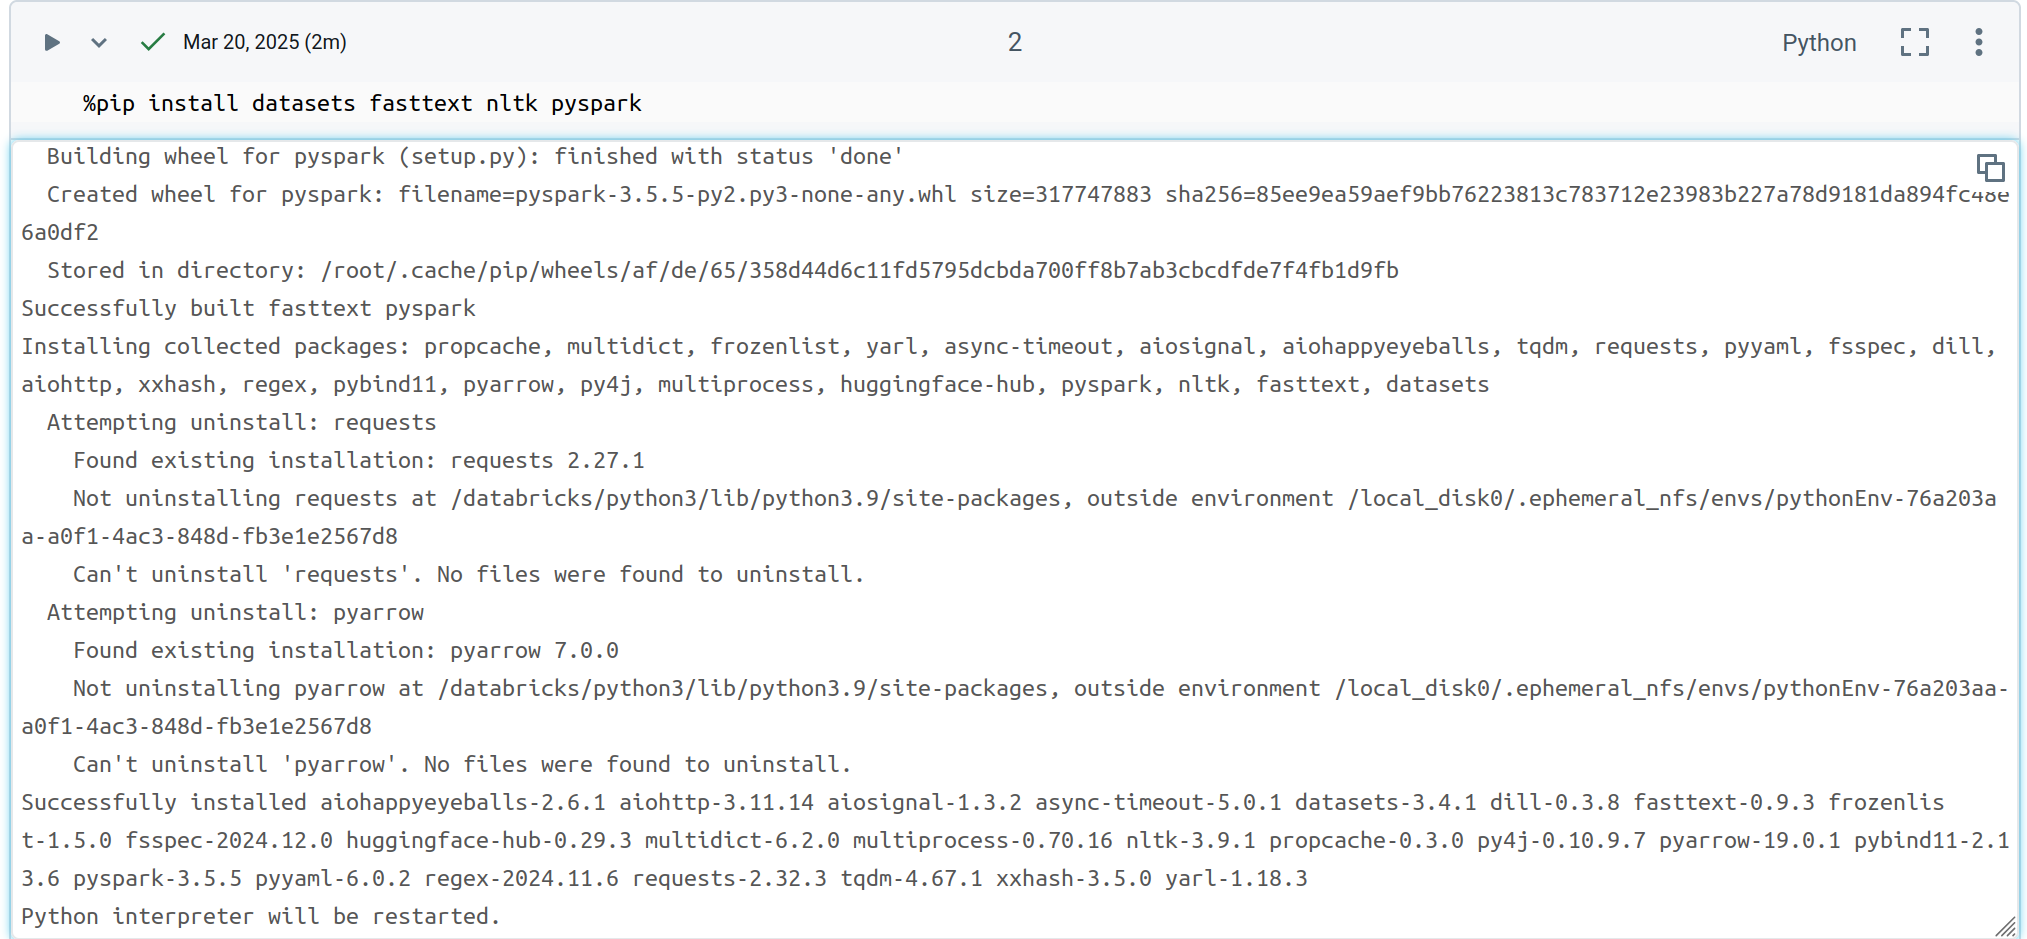
\includegraphics[width=0.6\textwidth]{evidencias/evidencia1.png}
    \caption{Instalando as bibbliotecas necessárias.}
    \label{fig:exemplo}
\end{figure}

\begin{figure}[htbp]
    \centering
    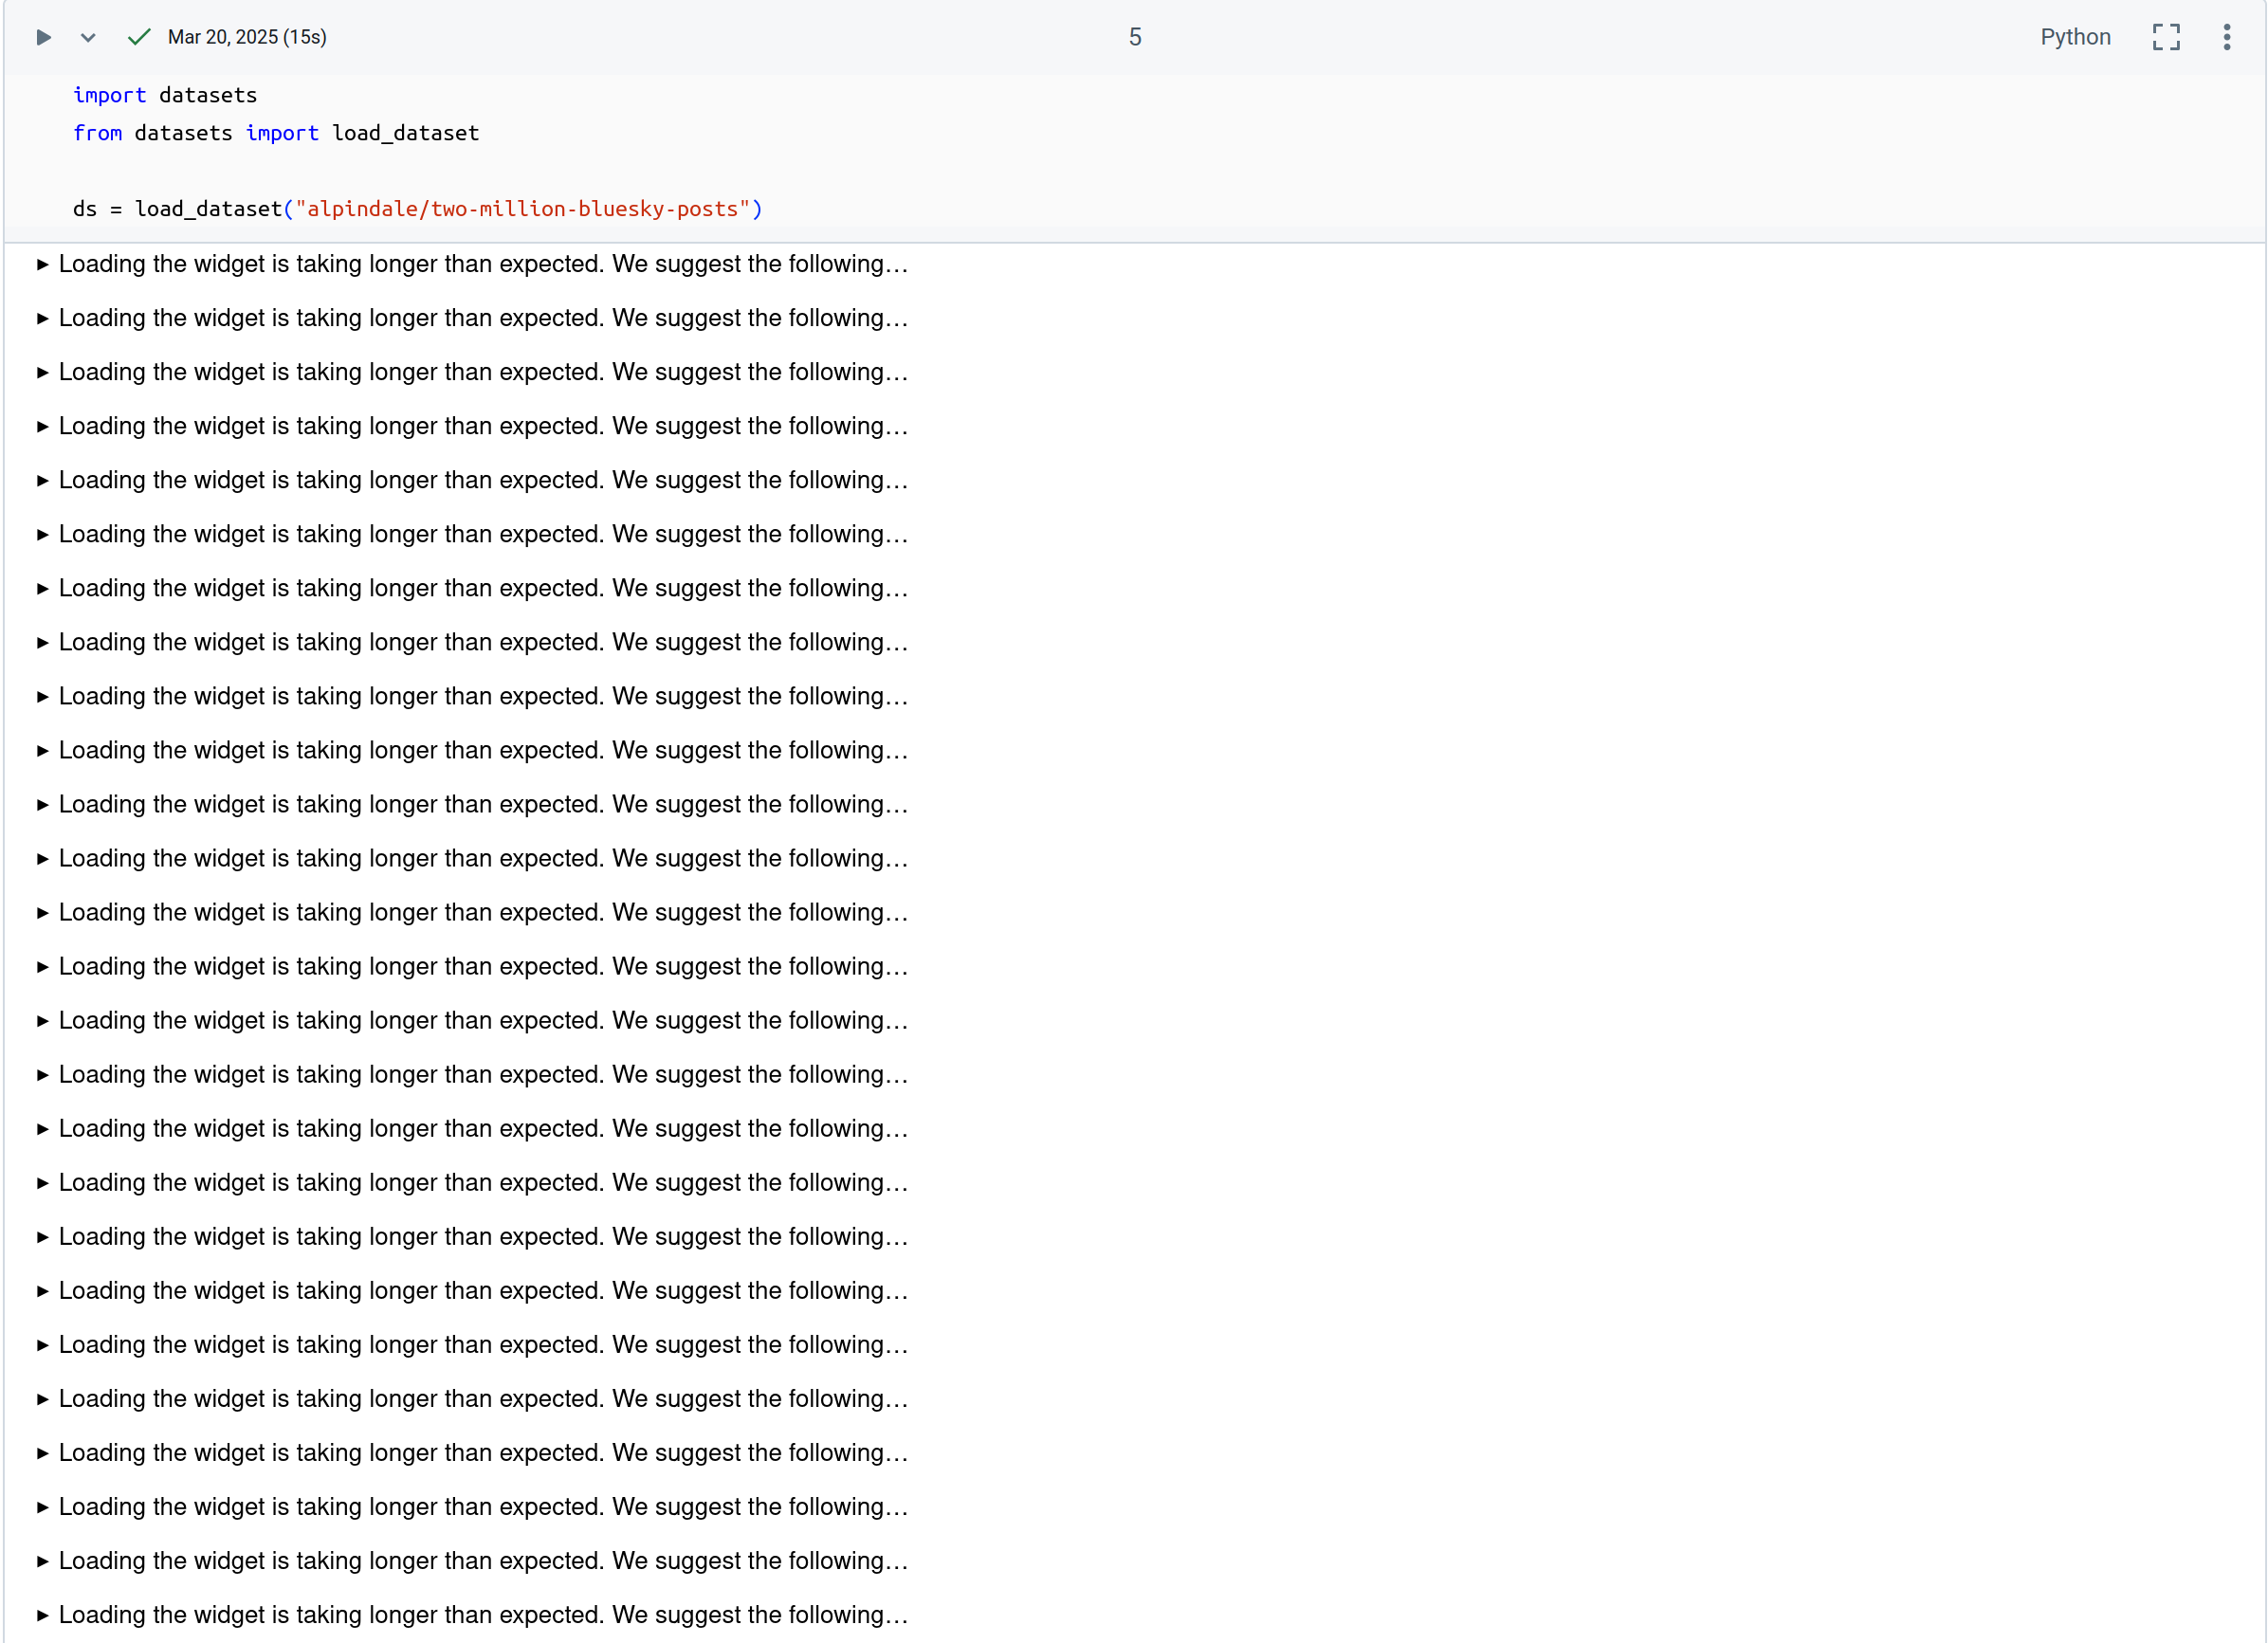
\includegraphics[width=0.6\textwidth]{evidencias/evidencia2.png}
    \caption{Carregando os datasets.}
    \label{fig:exemplo}
\end{figure}

\begin{figure}[htbp]
    \centering
    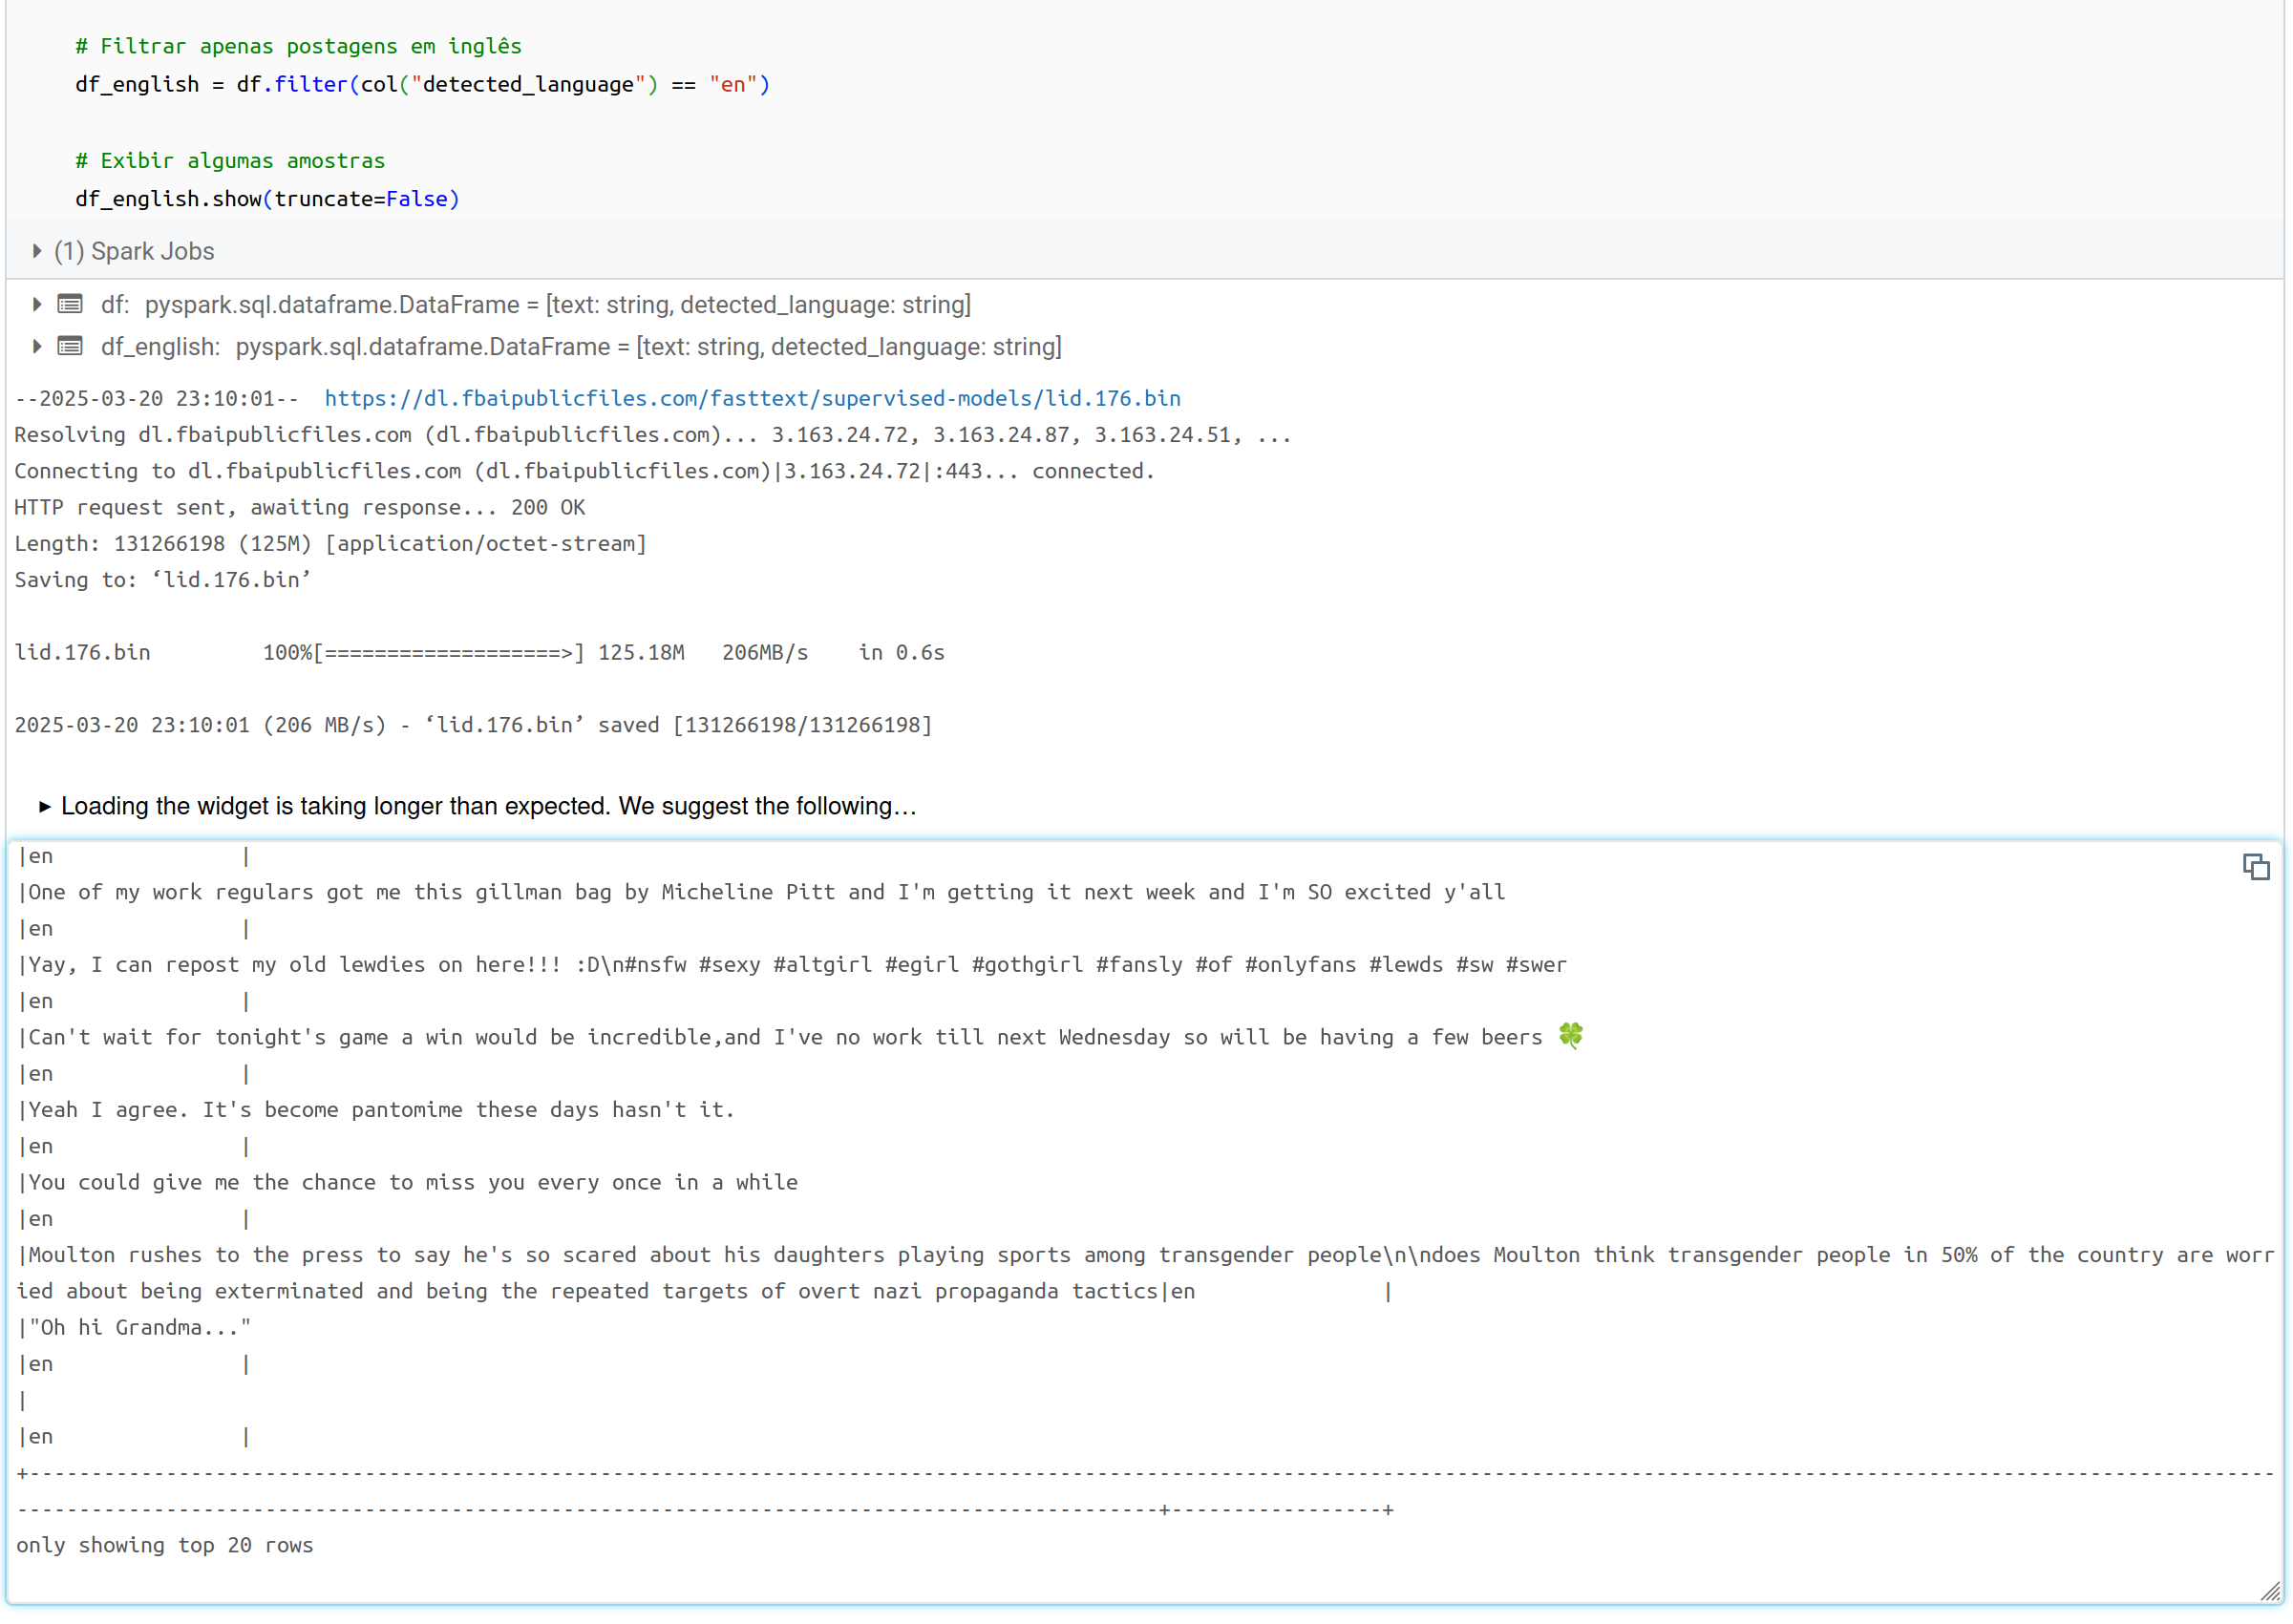
\includegraphics[width=0.6\textwidth]{evidencias/evidencia3.png}
    \caption{Extração.}
    \label{fig:exemplo}
\end{figure}

\begin{figure}[htbp]
    \centering
    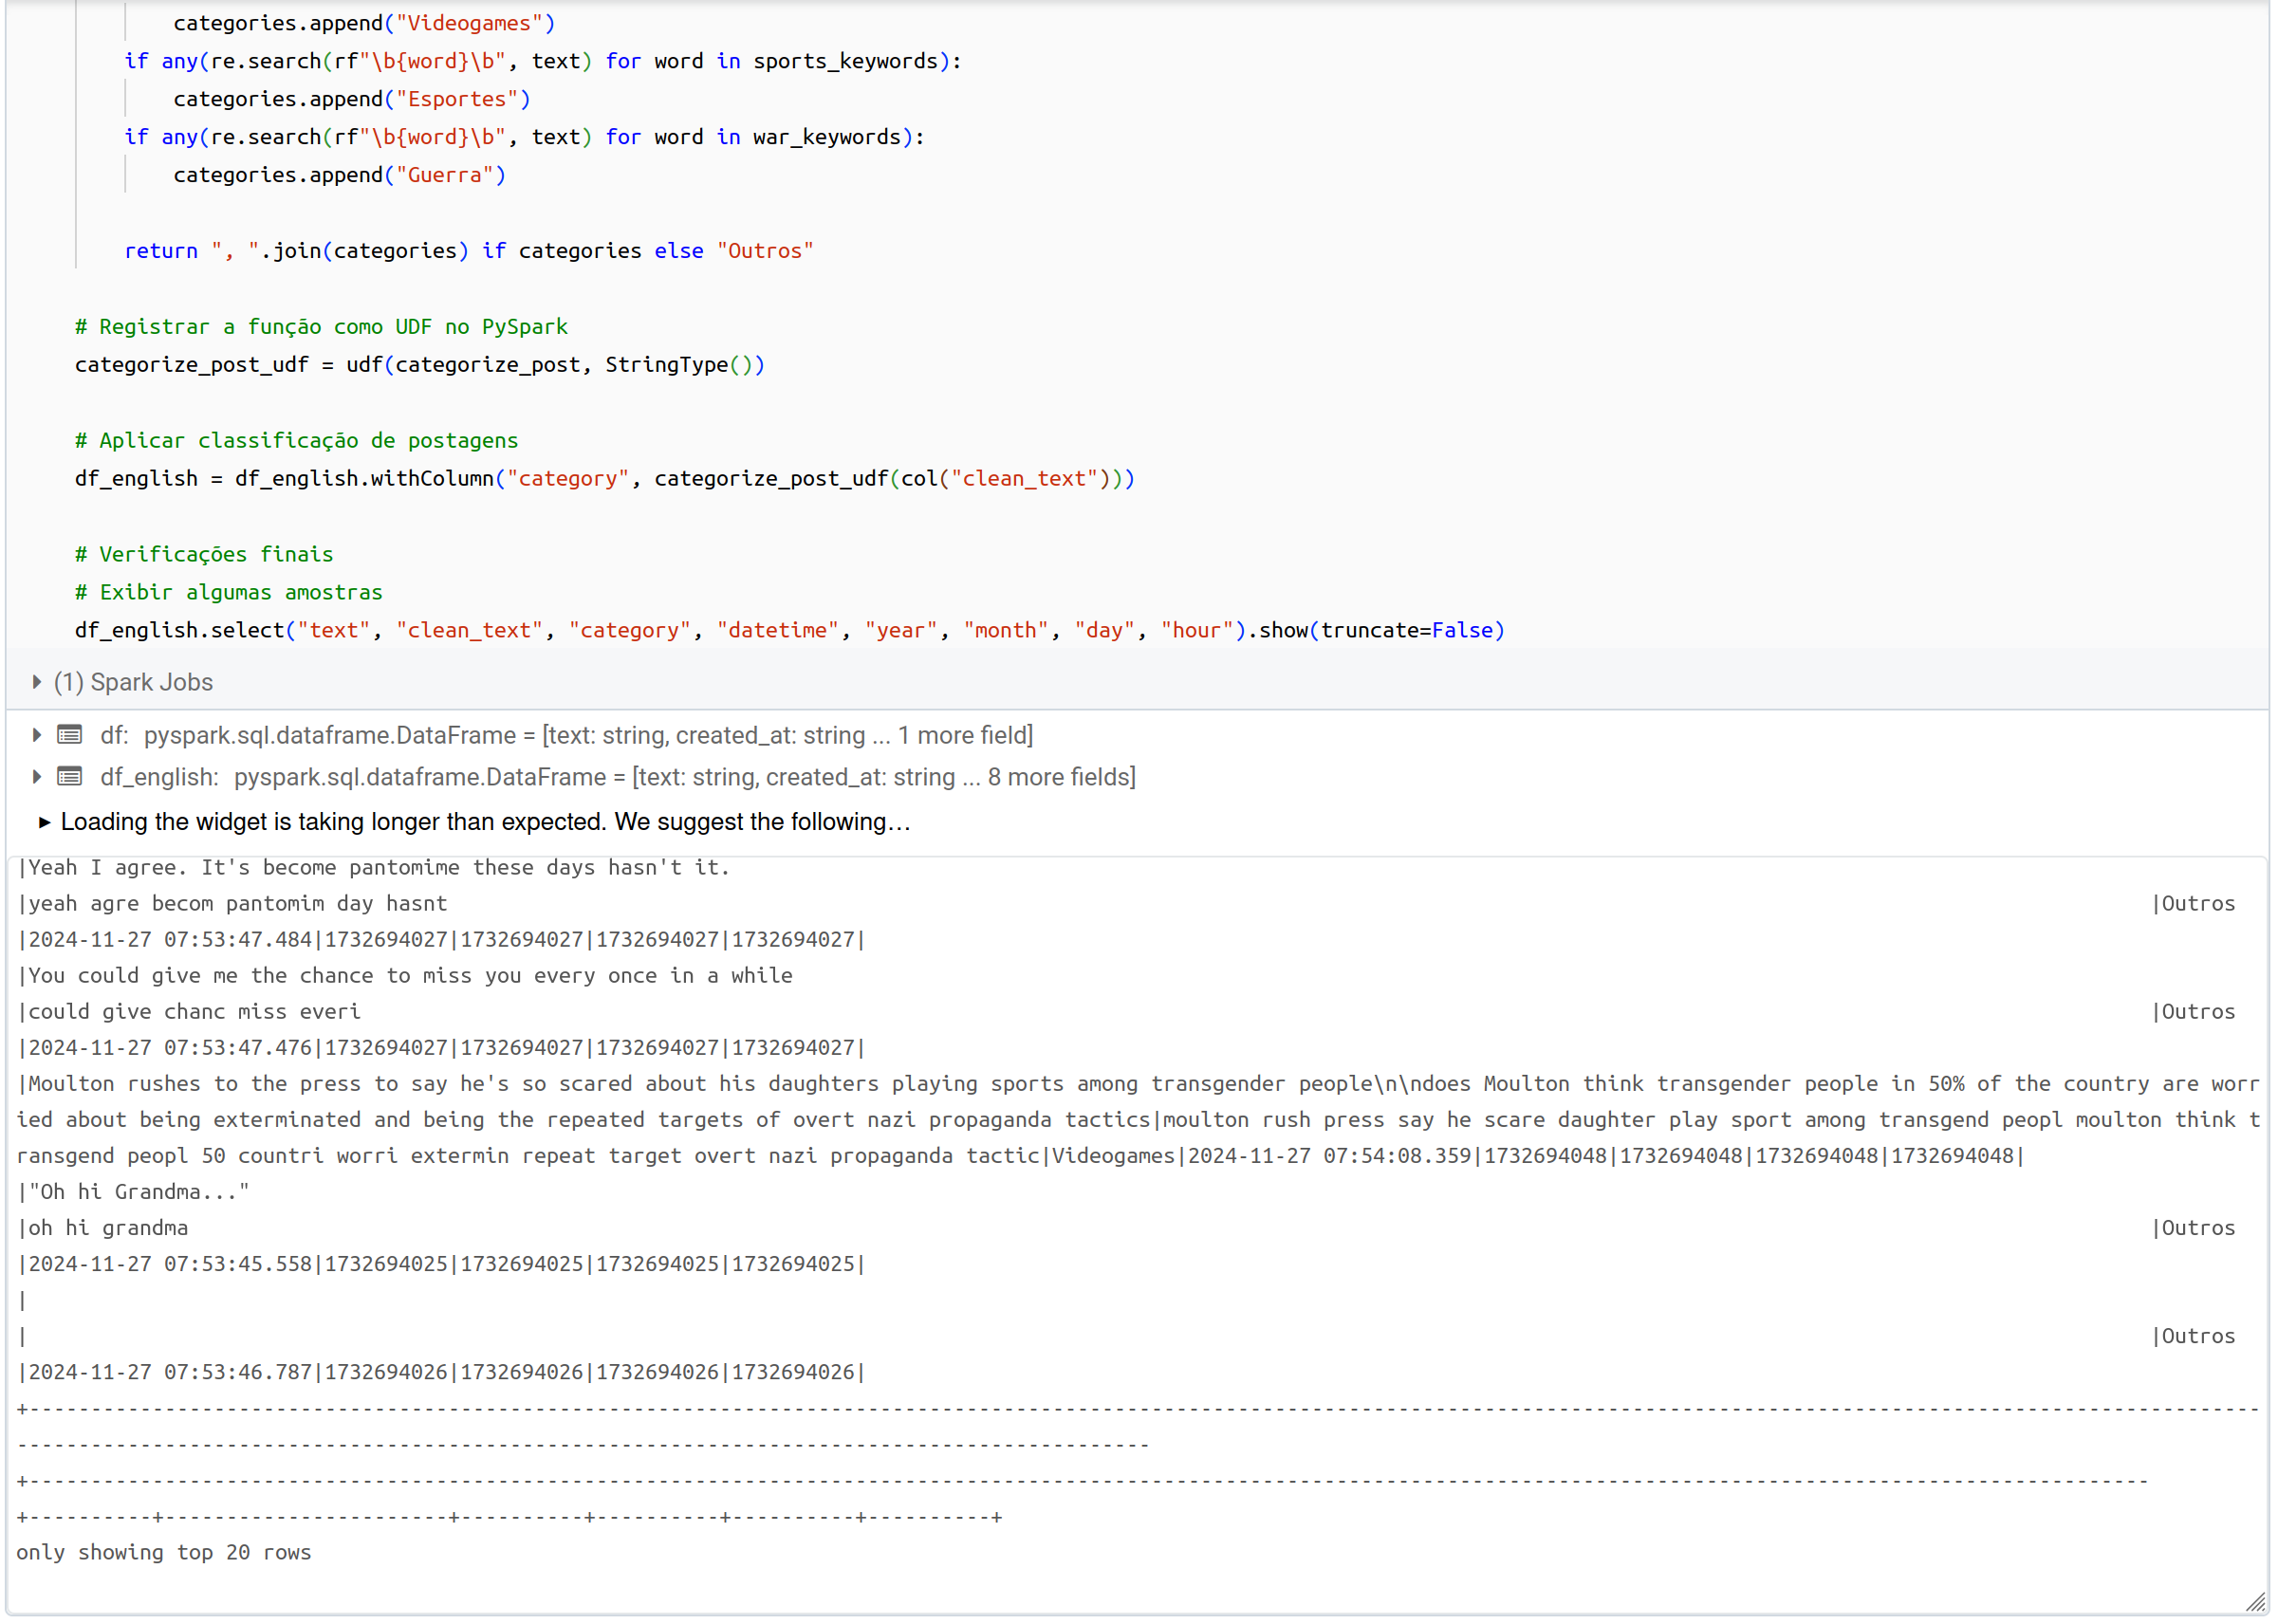
\includegraphics[width=0.6\textwidth]{evidencias/evidencia4.png}
    \caption{Transformação.}
    \label{fig:exemplo}
\end{figure}

\begin{figure}[htbp]
    \centering
    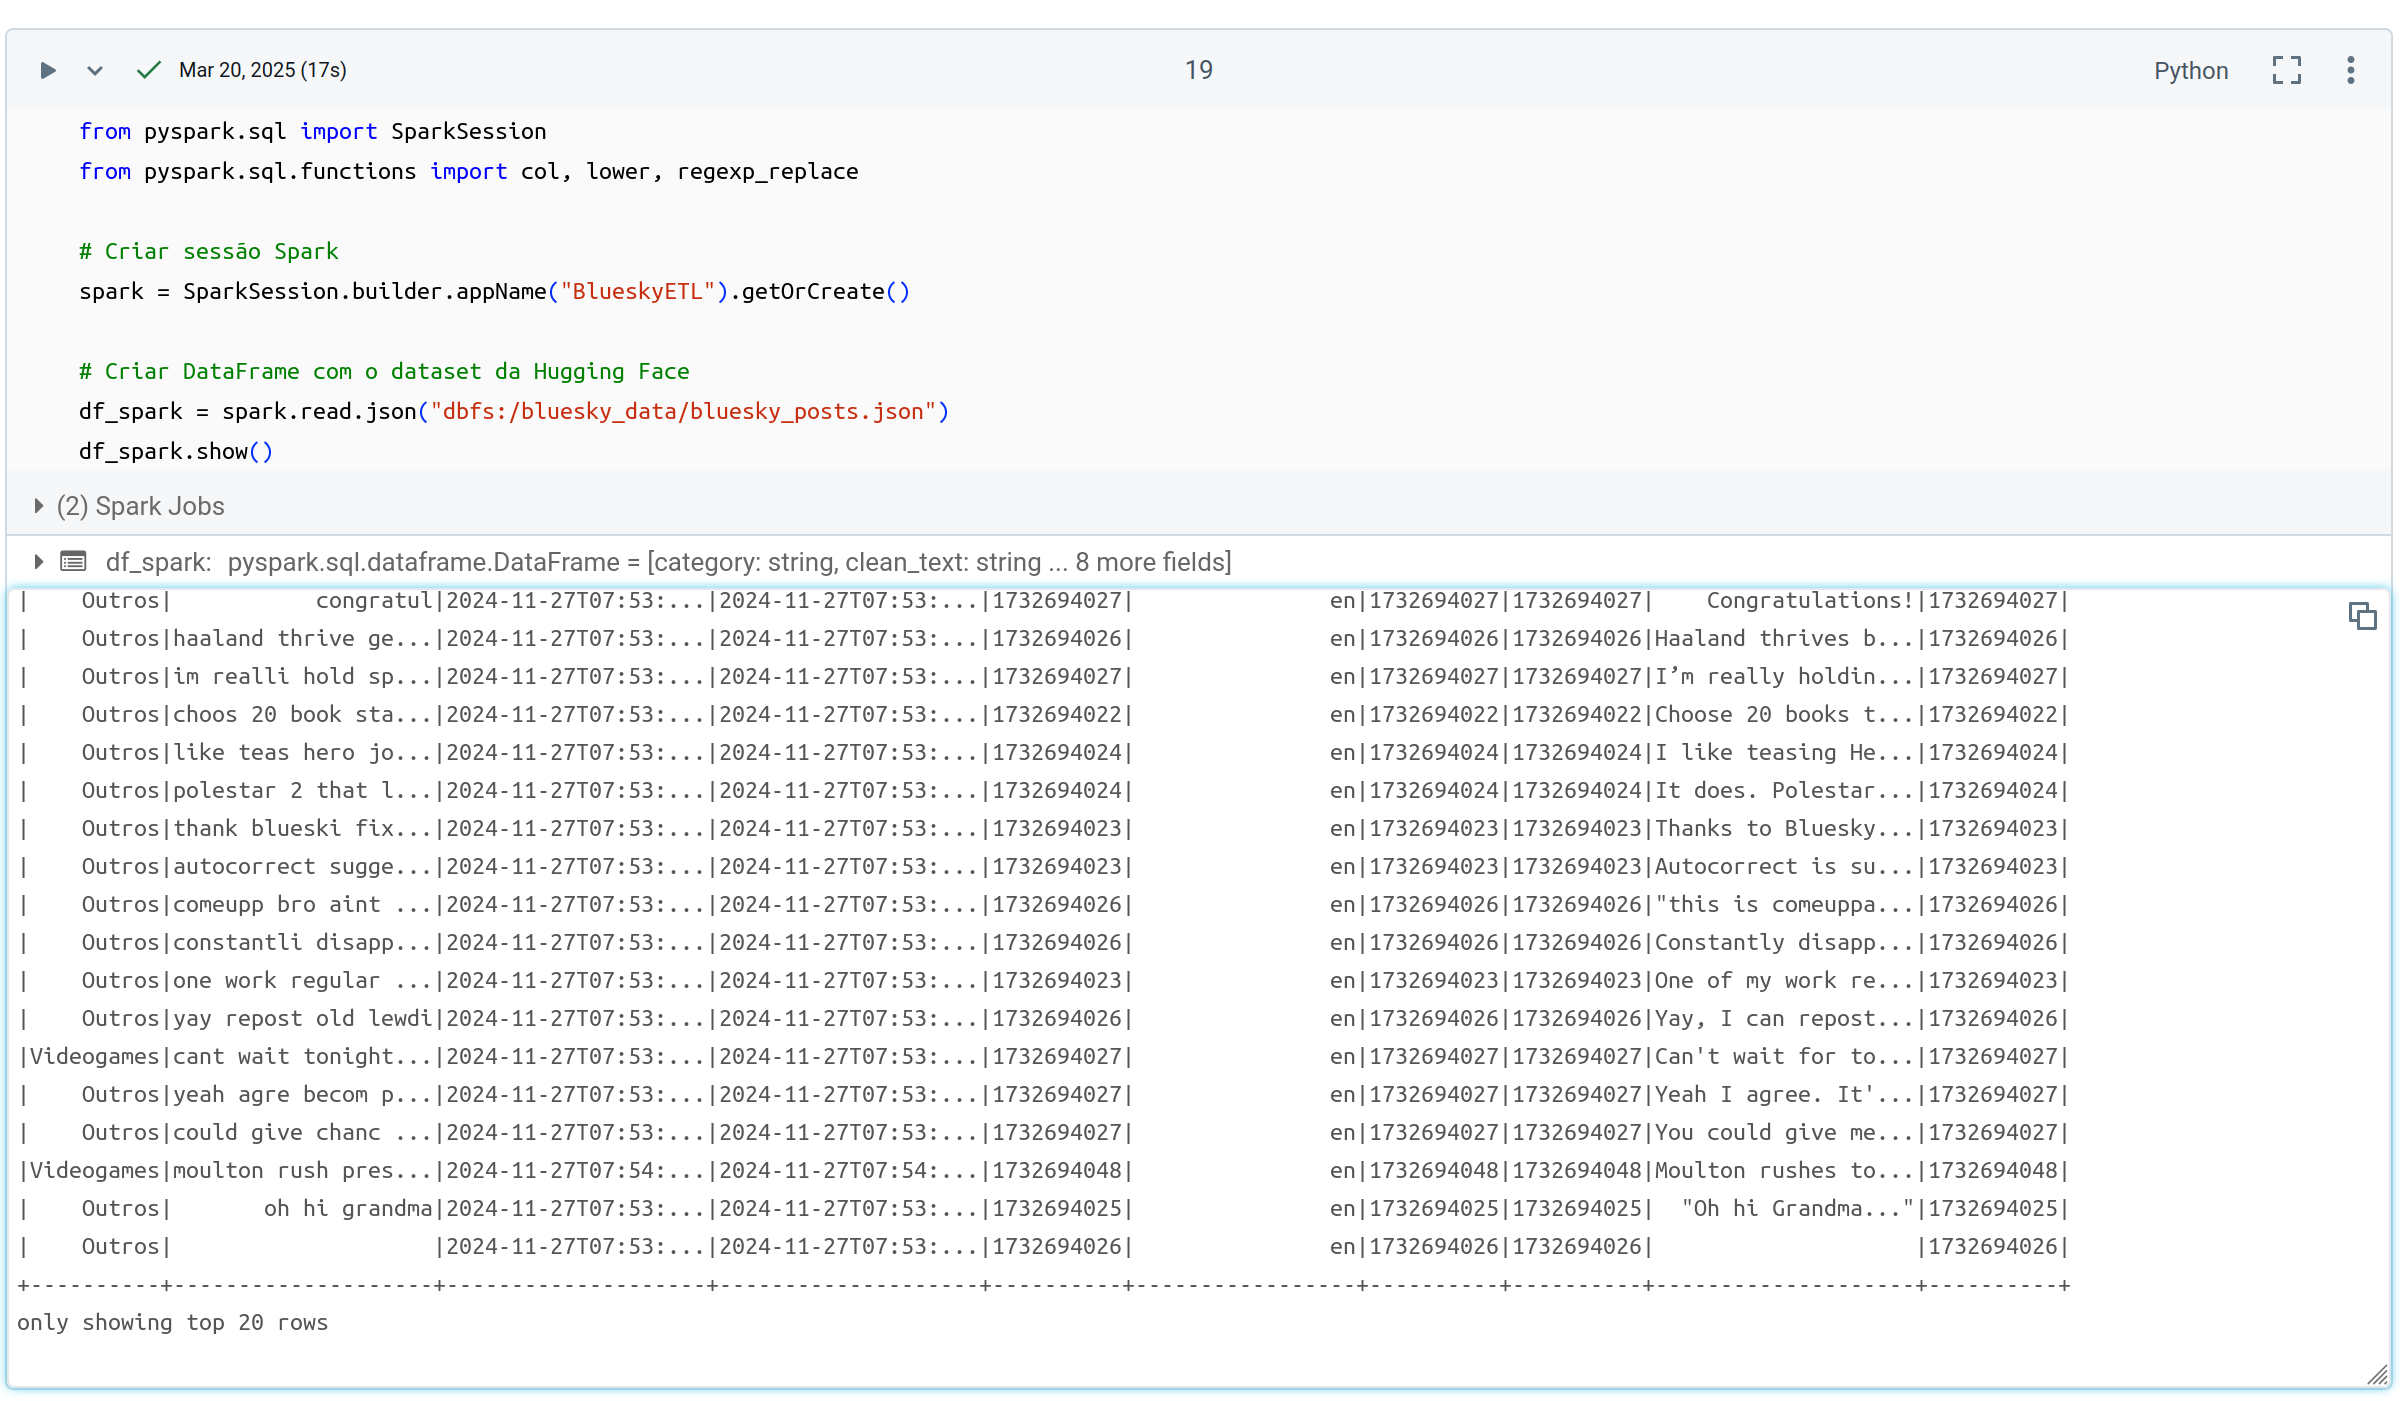
\includegraphics[width=0.6\textwidth]{evidencias/evidencia5.png}
    \caption{Carregamento, criando um DataFrame.}
    \label{fig:exemplo}
\end{figure}

\begin{figure}[htbp]
    \centering
    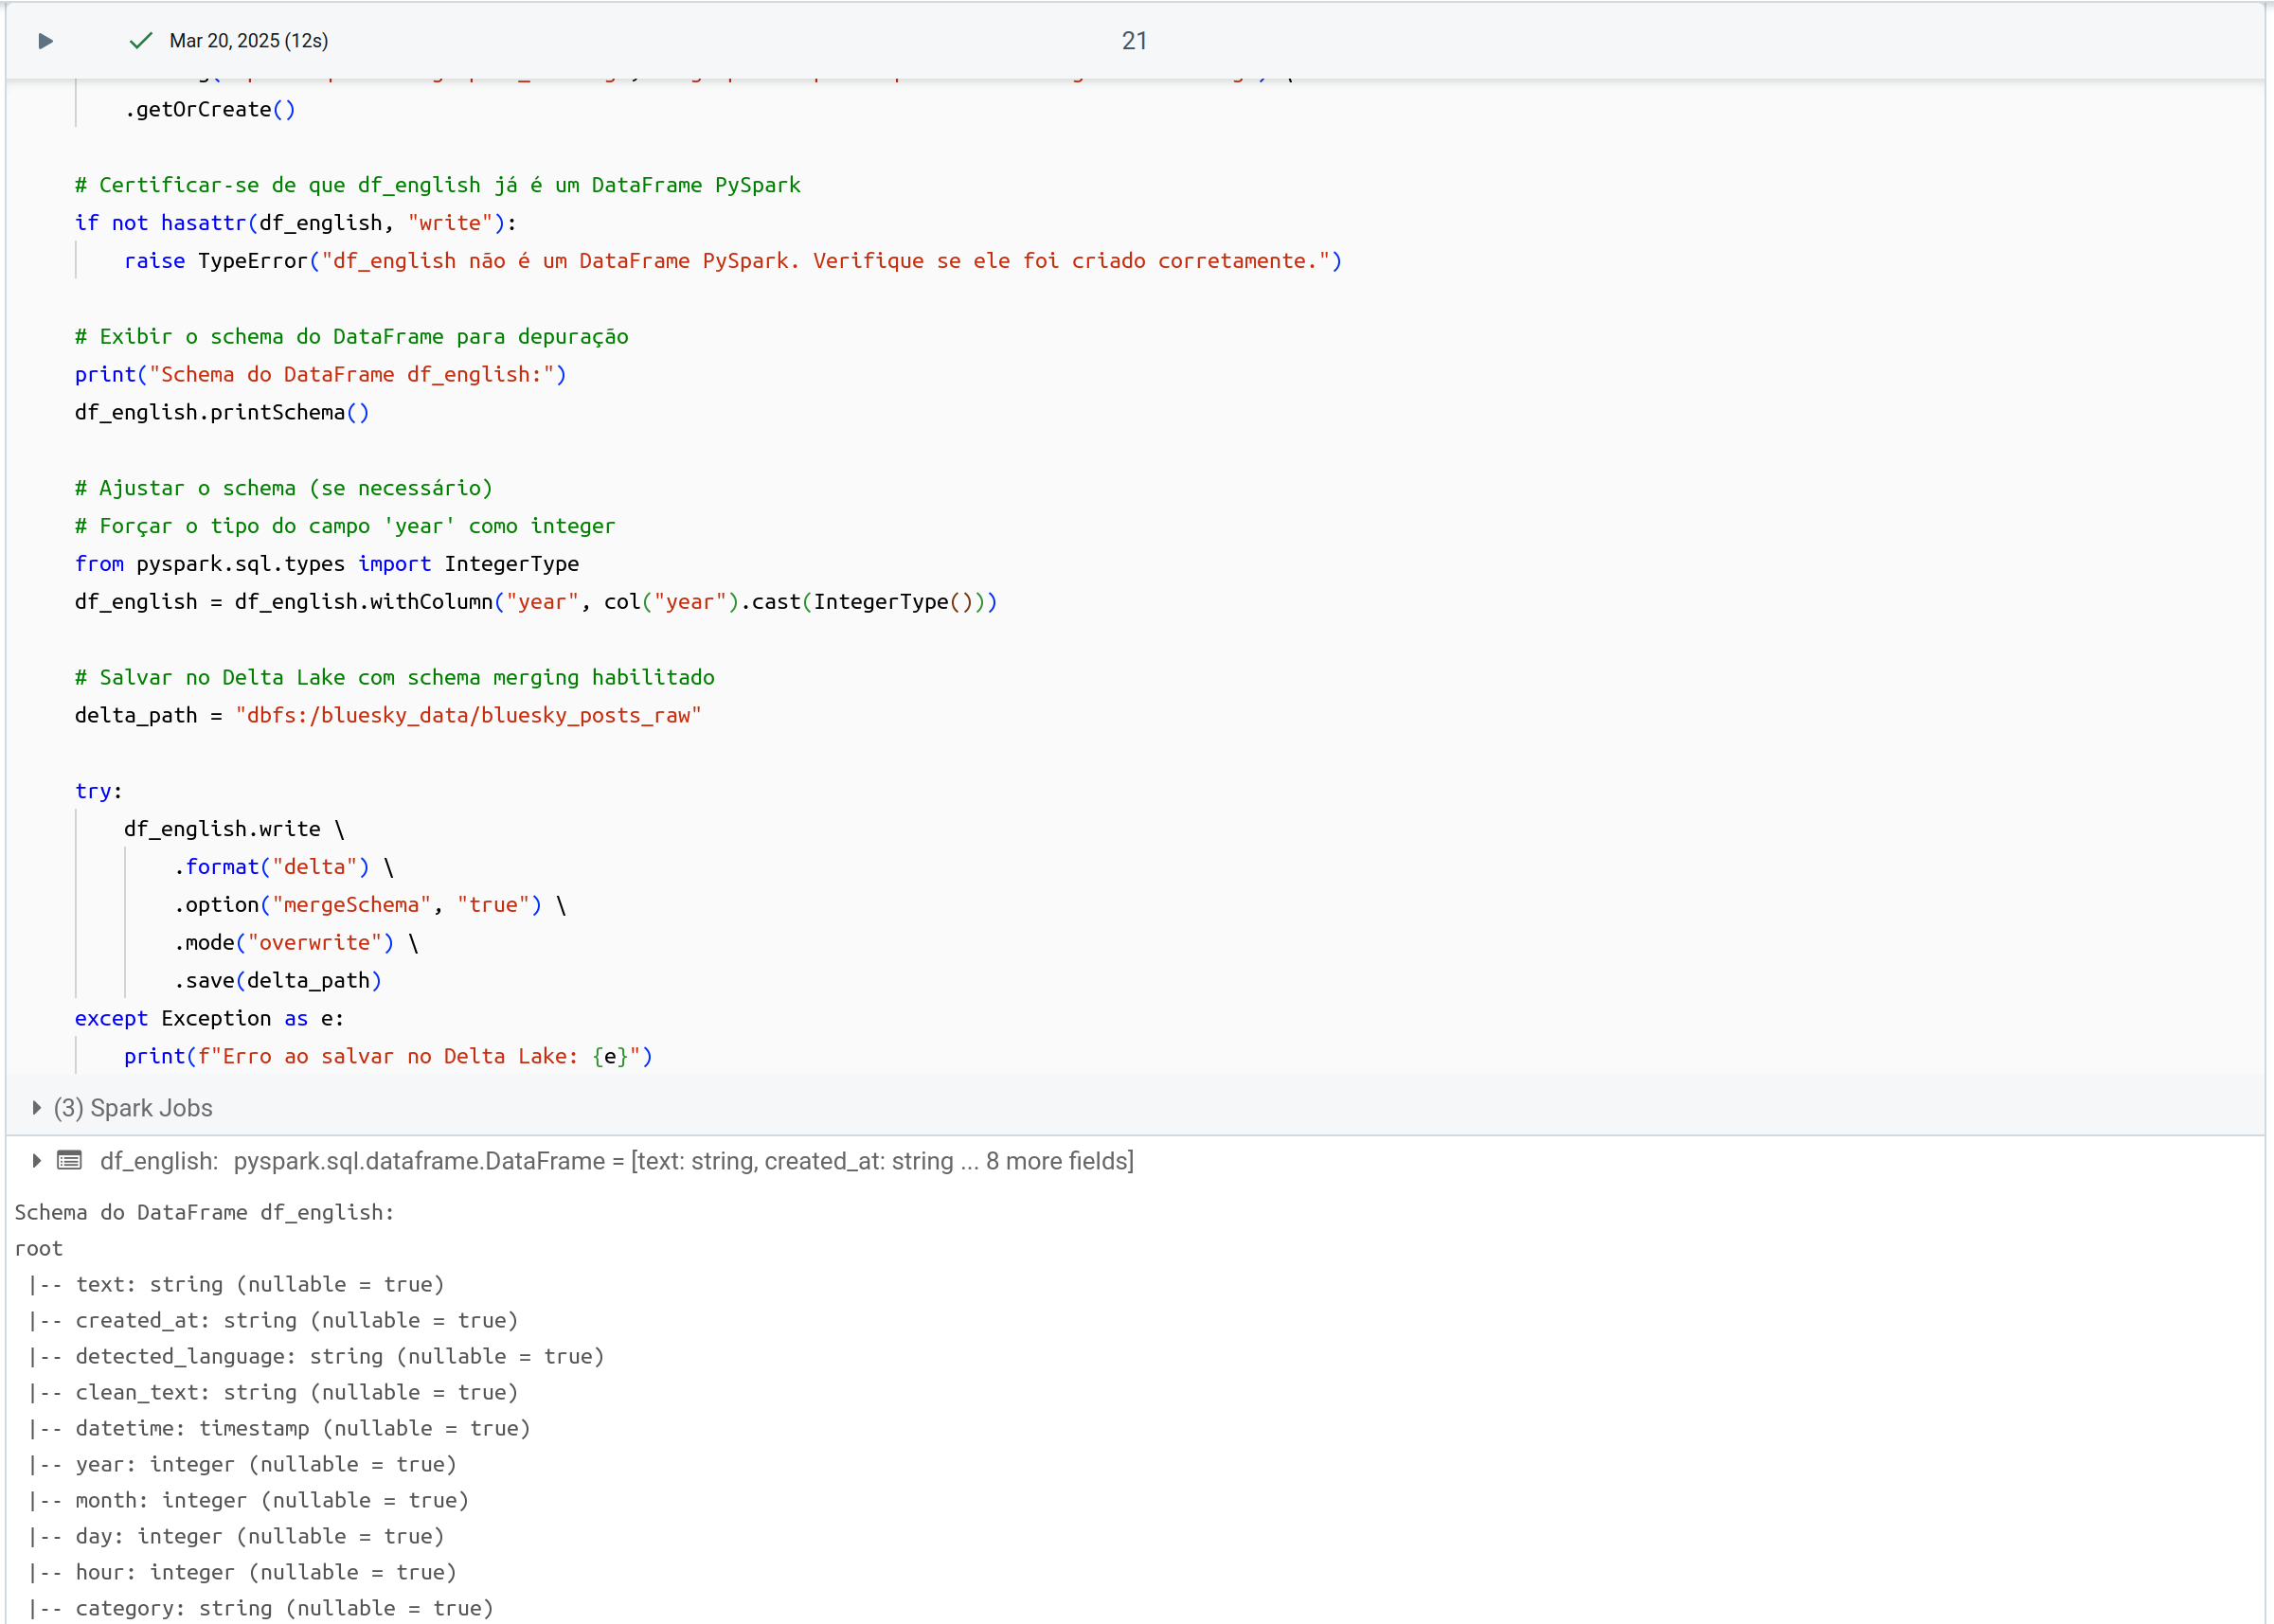
\includegraphics[width=0.6\textwidth]{evidencias/evidencia6.png}
    \caption{Carregamento, salvando no Delta Lake.}
    \label{fig:exemplo}
\end{figure}

\begin{figure}[htbp]
    \centering
    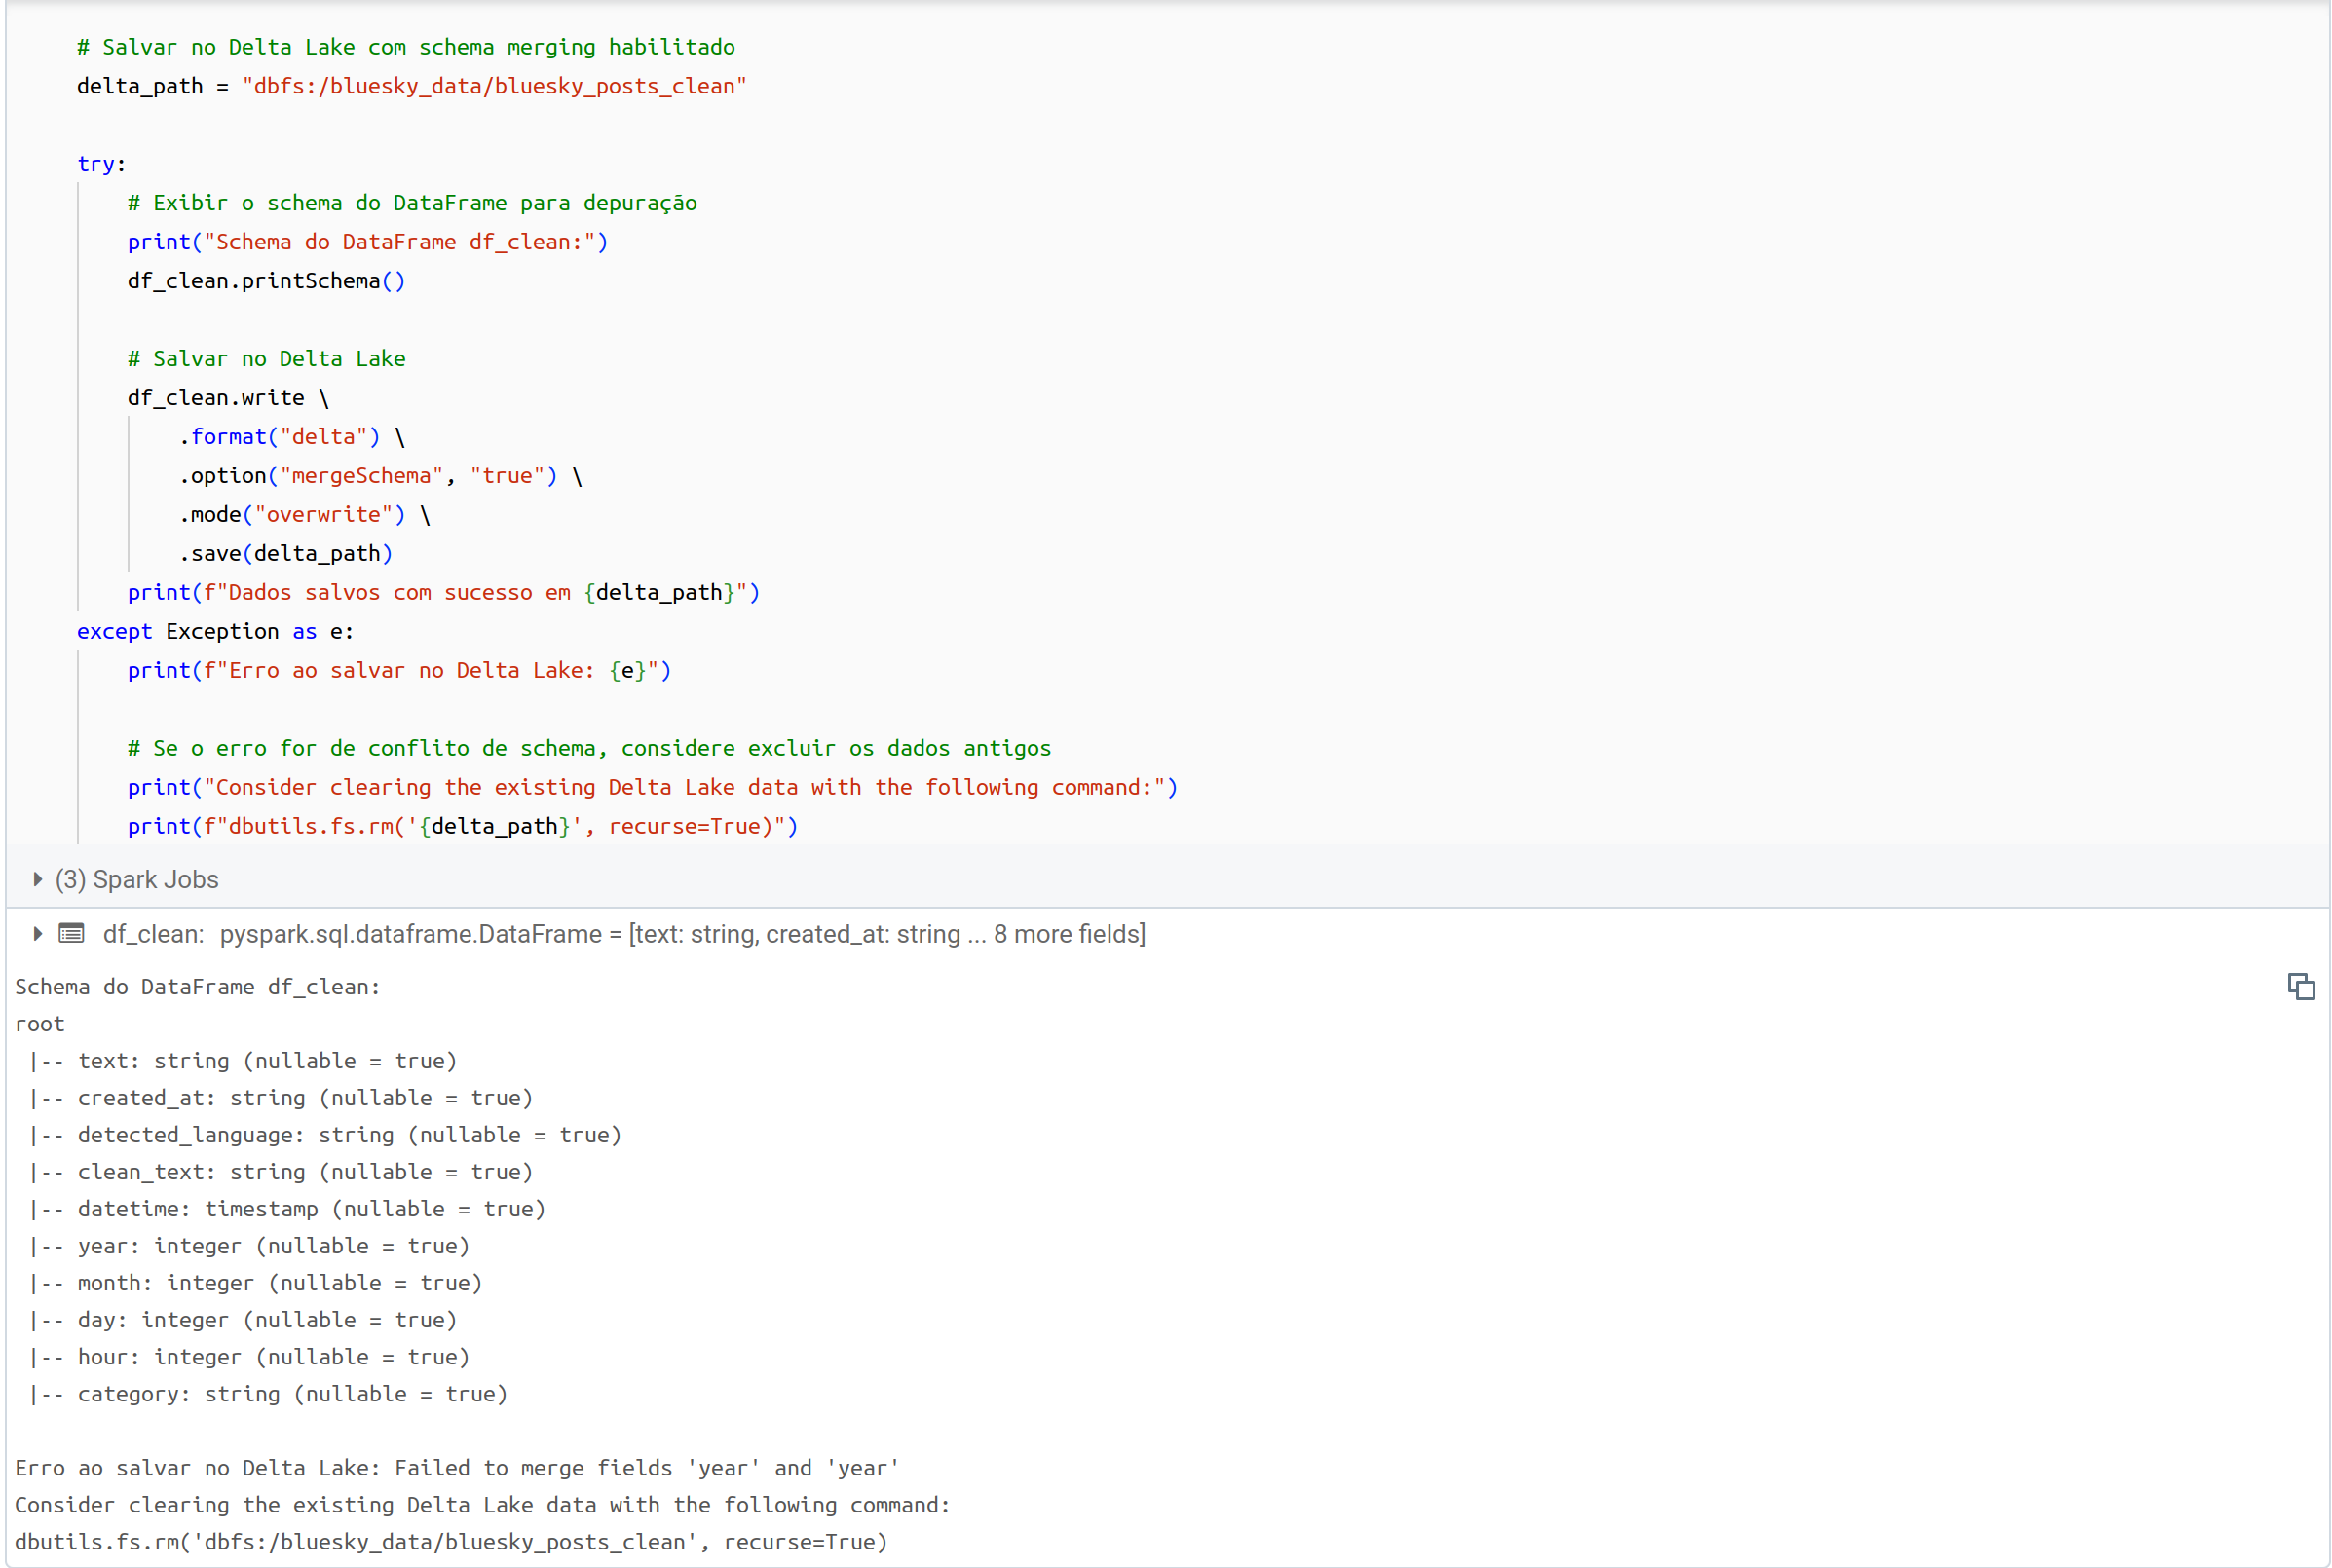
\includegraphics[width=0.6\textwidth]{evidencias/evidencia7.png}
    \caption{Carregamento, criação de uma Tabela Delta.}
    \label{fig:exemplo}
\end{figure}

\begin{figure}[htbp]
    \centering
    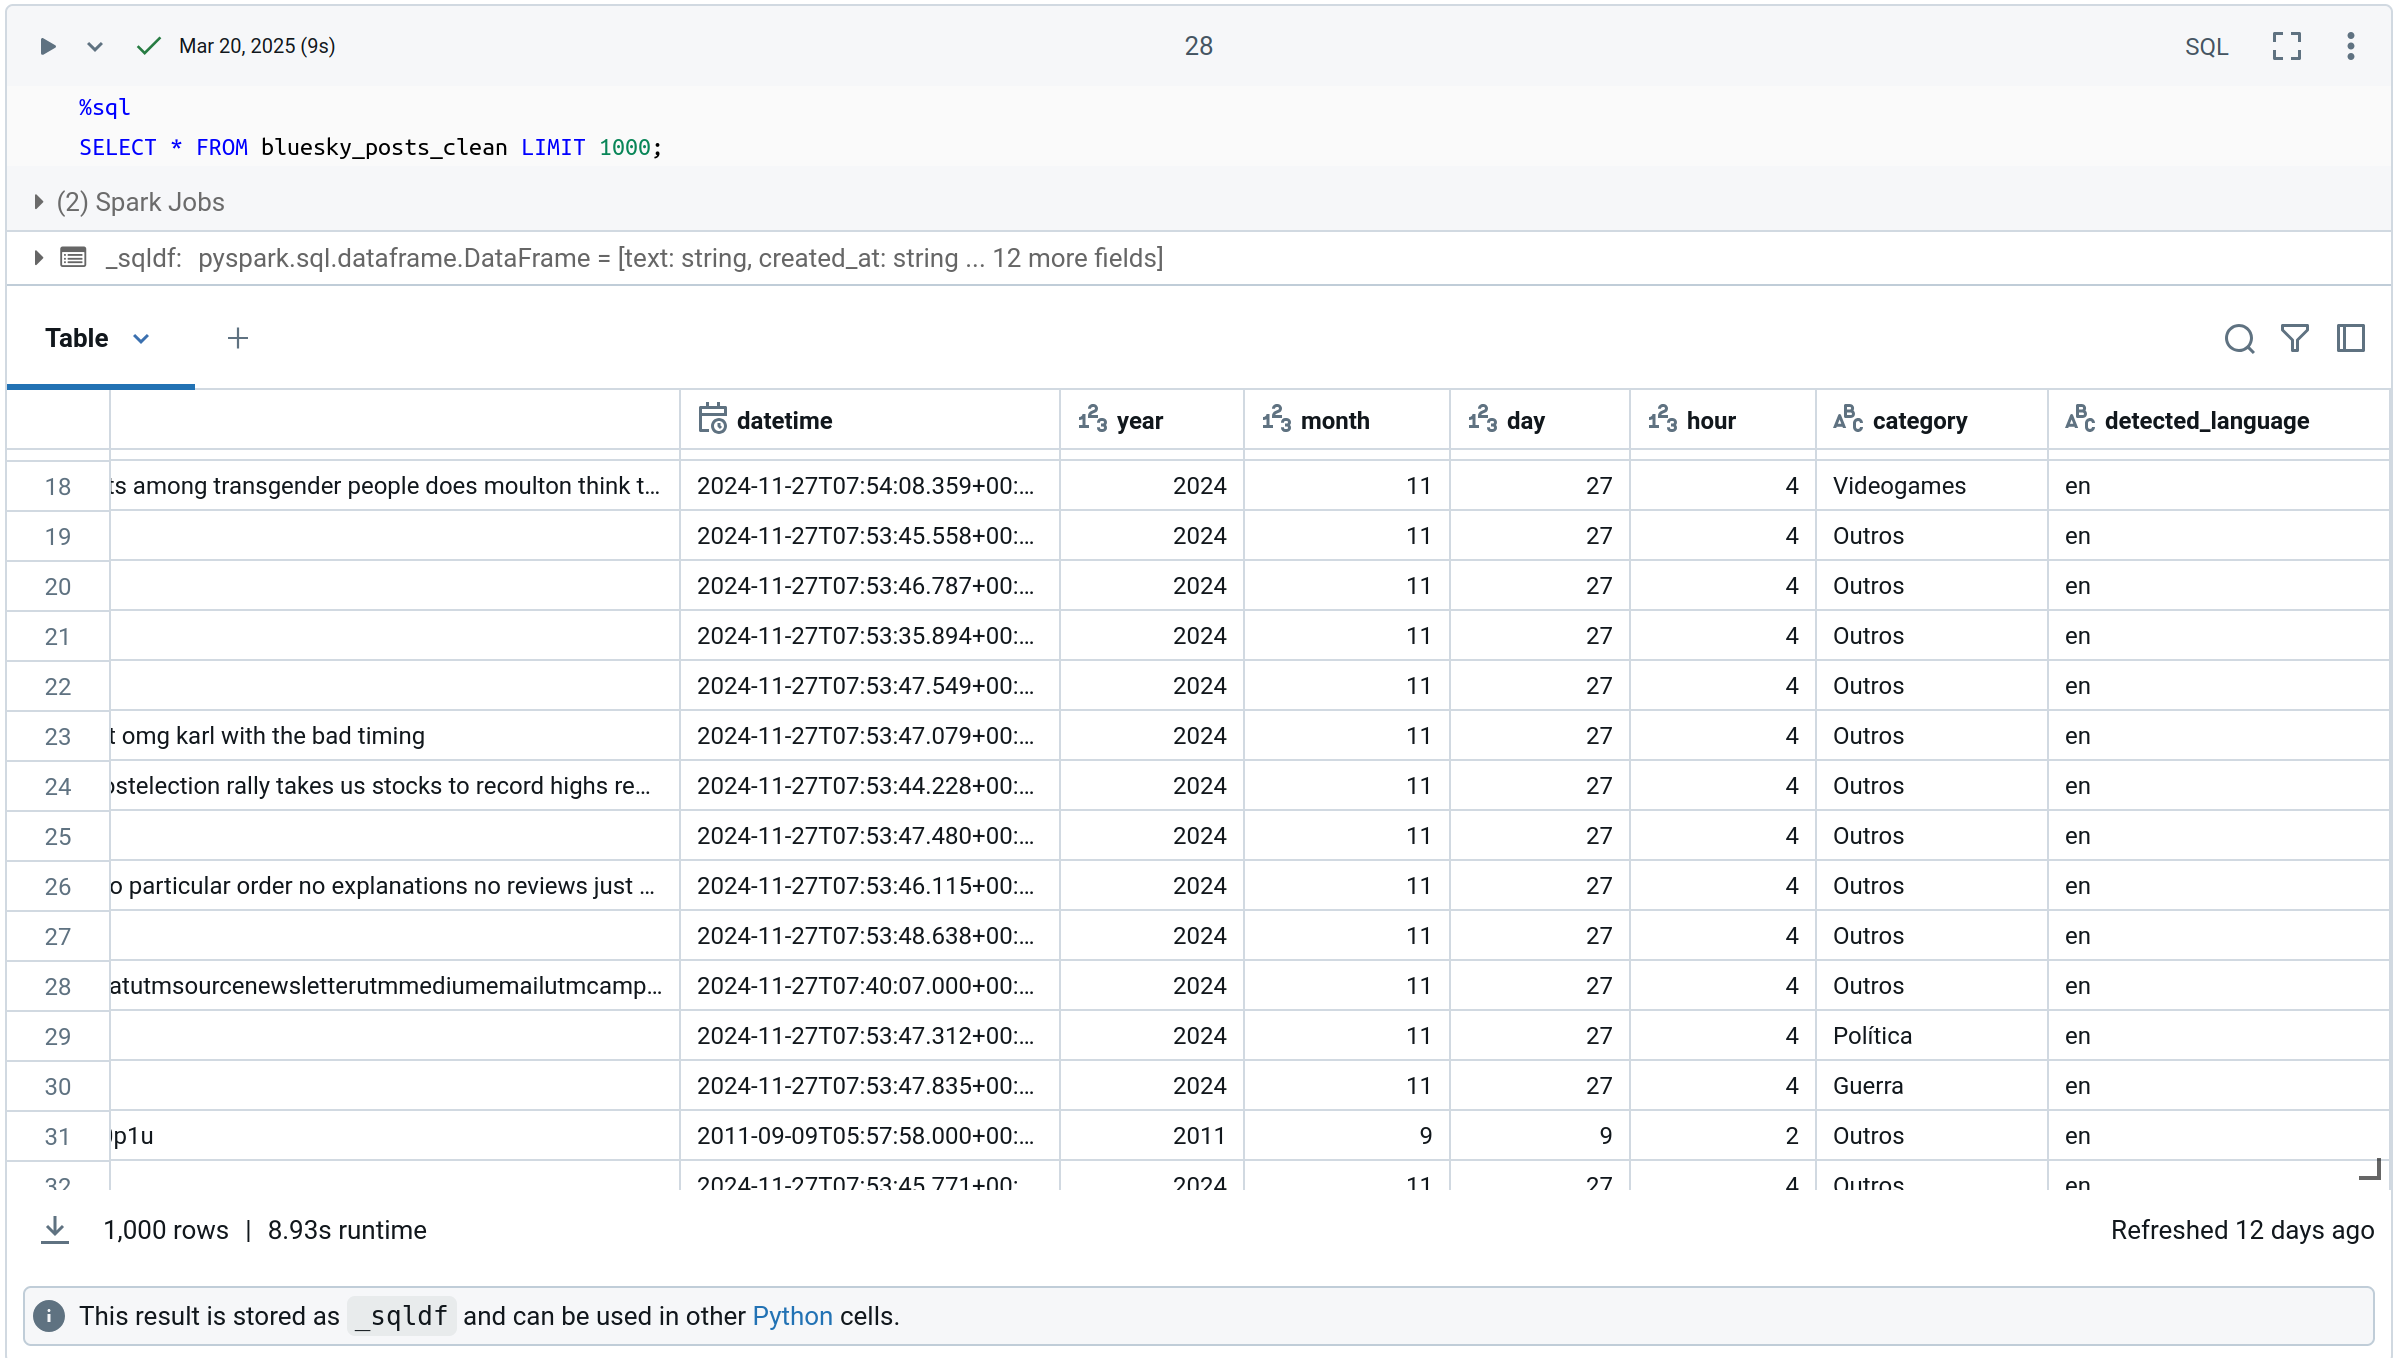
\includegraphics[width=0.6\textwidth]{evidencias/evidencia8.png}
    \caption{Carregamento, criação de uma tabela no Databricks SQL.}
    \label{fig:exemplo}
\end{figure}


\printindex

\end{document}